\subsubsection*{Оценка моделей по критериям}

\begin{center}
    Таблица 2. Оценка всех моделей проекта в соответствии с заявленными критериями
\end{center}

\begin{center}
    \textbf{Модель №1}
\end{center}

\begin{longtable}{|p{4cm}|p{2.5cm}|p{7.5cm}|}
    \hline
    \multicolumn{3}{|c|}{\textbf{Оригинальное здание} } \\
    \hline
    \multicolumn{3}{|c|}{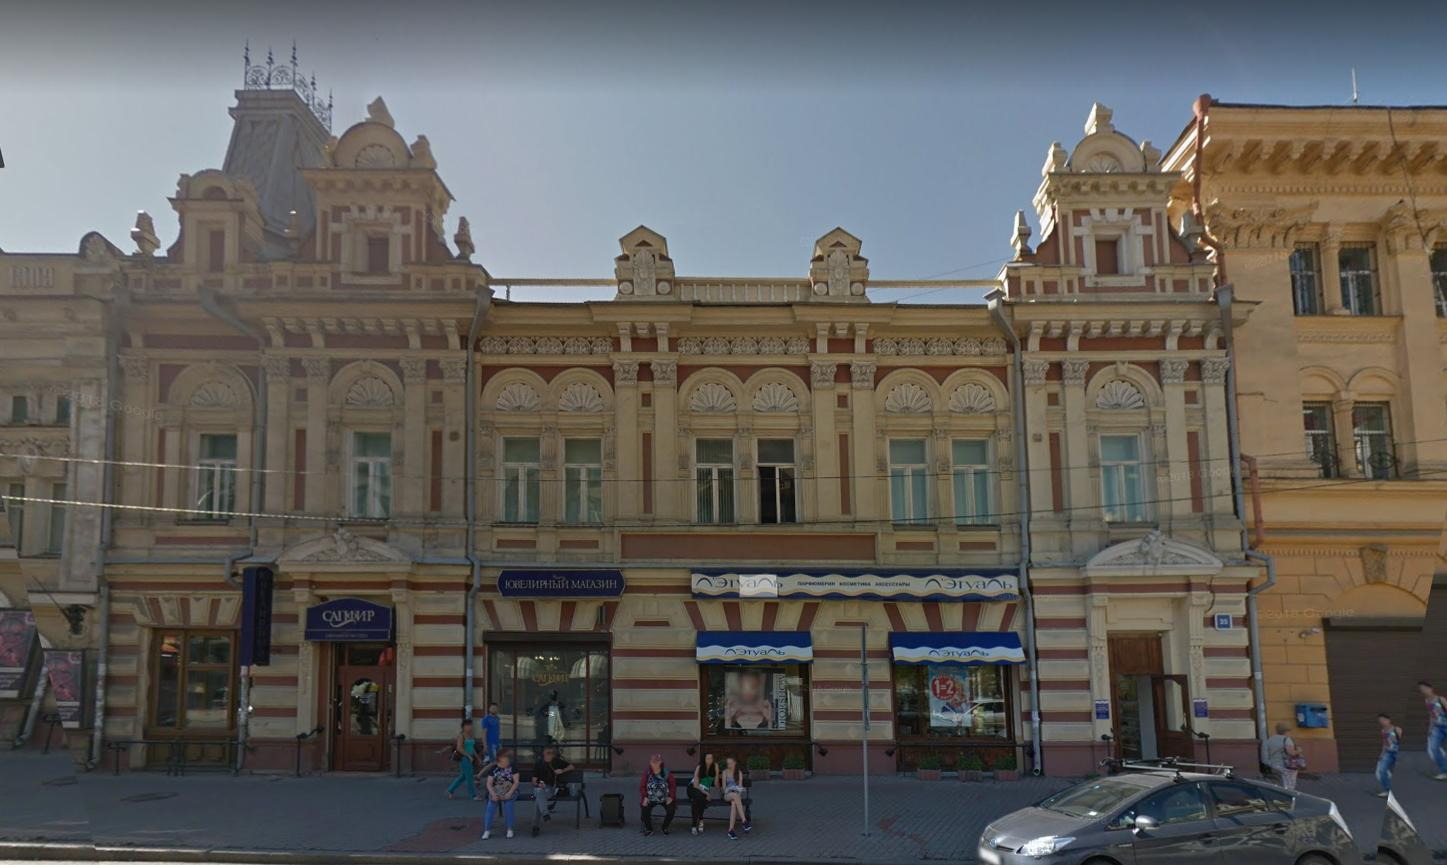
\includegraphics[width=11cm]{1}} \\
    \hline
    \multicolumn{3}{|c|}{\textbf{Модель}} \\
    \hline
    \multicolumn{3}{|c|}{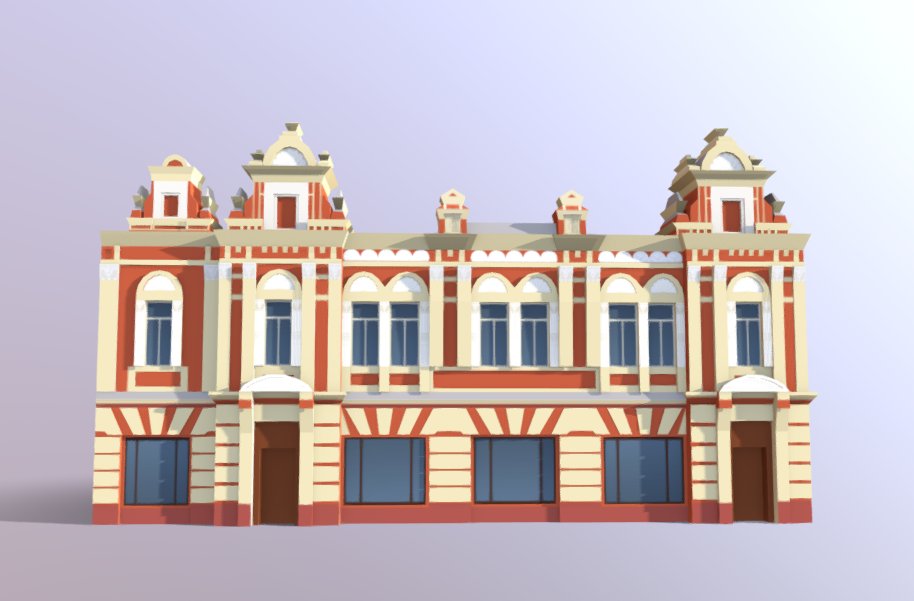
\includegraphics[width=11cm]{src/model_1}} \\
    \hline
    \textbf{Критерий} & \textbf{Балл/ Max.балл} & \textbf{Комментарии} \\
    \hline
    Количество полигонов < 3k. & 0.9/0.9 & Количество полигонов - 2 695, соответствует допустимому диапазону. \\
    \hline
    Детализация. & 0.7/0.7 & Модель не является примитивом, отдельные части не перегружены лишними деталями, детализация не влияет на критерий количества полигонов. \\
    \hline
    Сходство с реальным объектом. & 0.7/0.7 & Объект можно легко опознать при сравнении с оригиналом - сохранены общие пропорции здания, характерные детали и количественный фактор (окна, двери и т.п.) \\
    \hline
    UV-развертка. & 0.6/0.6 & Развертка присутствует. Вес развертки правильный (окрашена в равномерный синий цвет без ярких зеленых или желтых зон).

    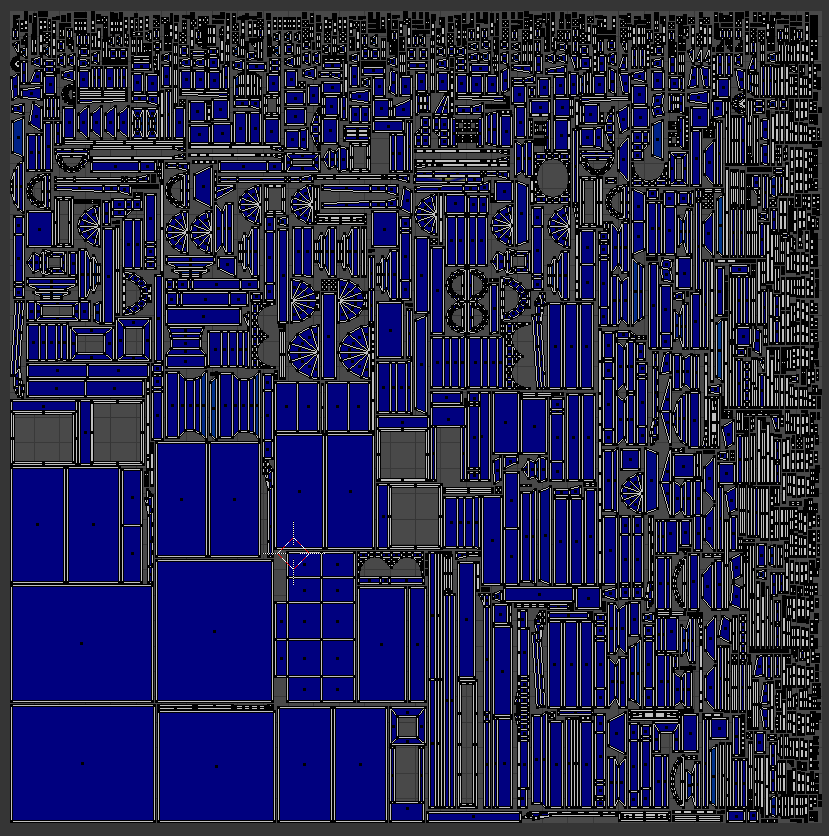
\includegraphics[width=7cm]{src/uv_1} \\
    \hline
    Наличие текстур. & 2.0/2.0 & Текстура присутствует (+ дополнительная текстура для ambient occlusion), все текстурные элементы запечены на одну текстуру.

    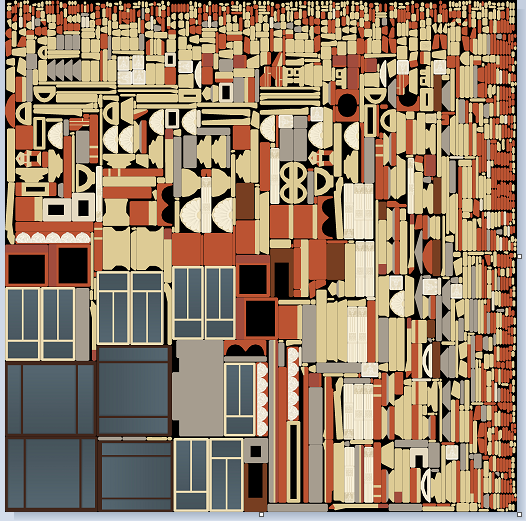
\includegraphics[width=7cm]{src/tec_1}\\
    & & 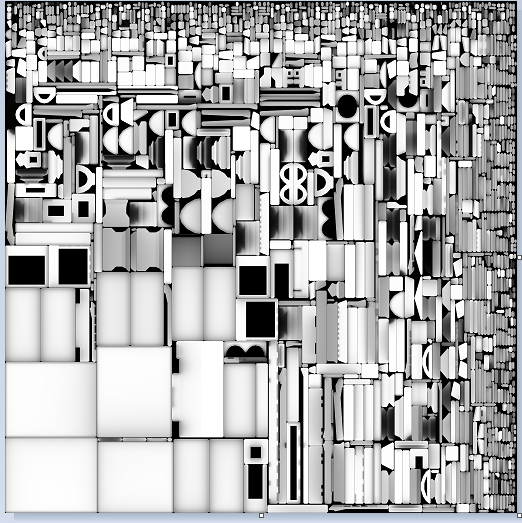
\includegraphics[width=7cm]{src/tec_2}\\
    \hline
    Отсутствие перевернутых нормалей. & 0.45/0.45 & Оси нормалей отображаются верно, направлены из объекта, а не вовнутрь. Нет затемненных участков меша или участков объекта без отображаемых текстур (свидетельство перевернутых нормалей).

    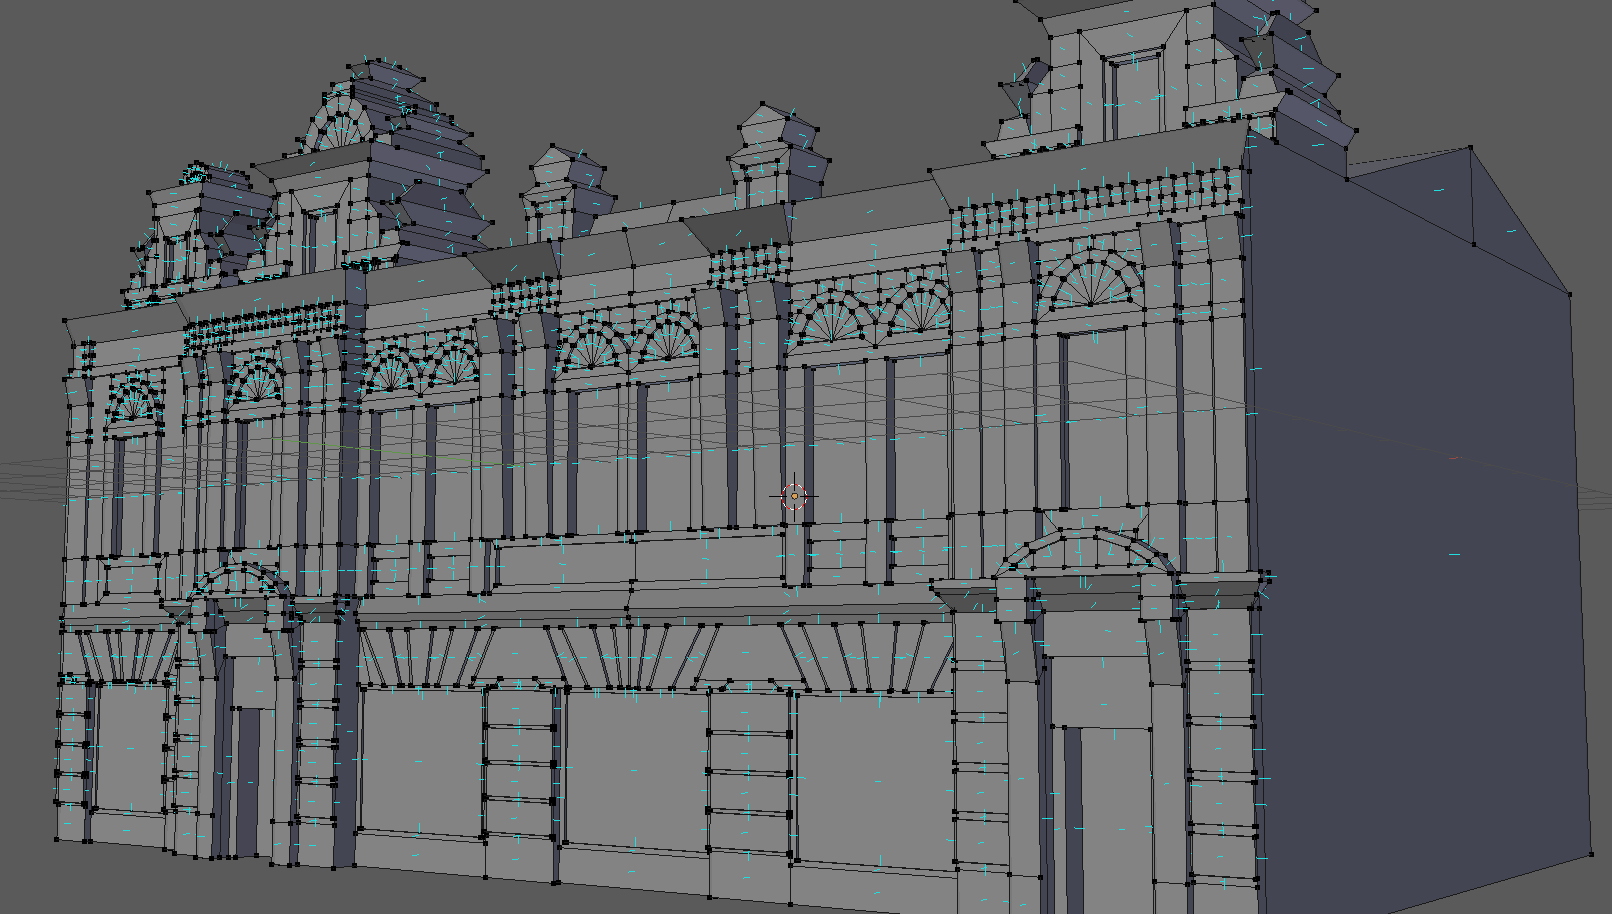
\includegraphics[width=7cm]{src/norm_1}\\
    & & 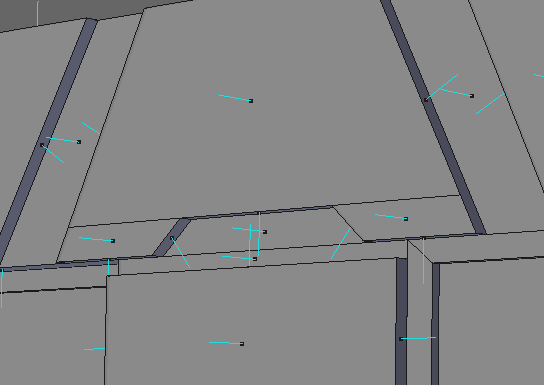
\includegraphics[width=7cm]{src/norm_2}\\
    \hline
    Отсутствие неправильных полигонов. & 0.6/0.6 & Все полигоны имеют форму четырехугольника или треугольника, нет полигонов с большим количеством углов. \\
    \hline
    \multicolumn{3}{|c|}{\textbf{Итого за модель: 5.95}} \\
    \hline
\end{longtable}

\begin{center}
    \textbf{Модель №2}
\end{center}

\begin{longtable}{|p{4cm}|p{2.5cm}|p{7.5cm}|}
    \hline
    \multicolumn{3}{|c|}{\textbf{Оригинальное здание} } \\
    \hline
    \multicolumn{3}{|c|}{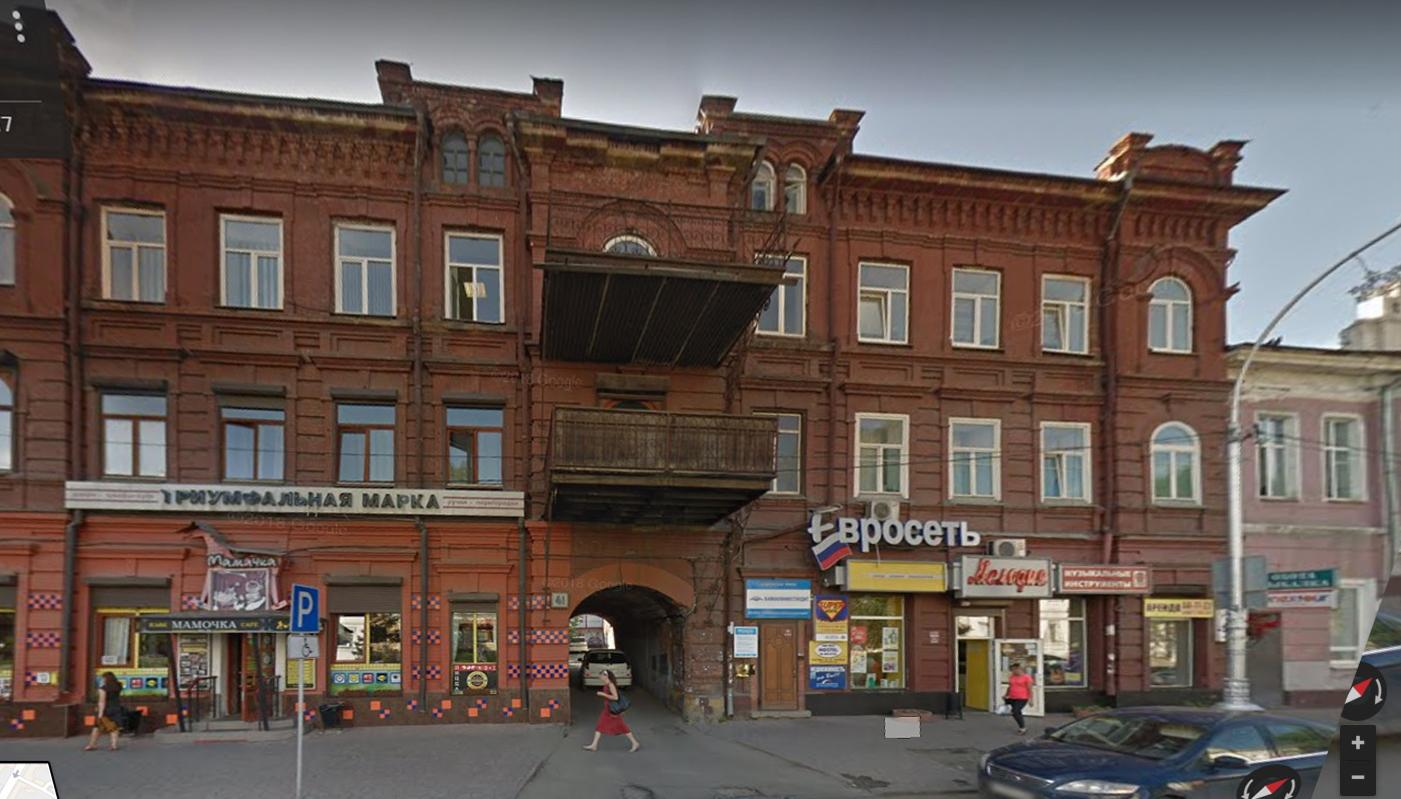
\includegraphics[width=11cm]{3}} \\
    \hline
    \multicolumn{3}{|c|}{\textbf{Модель}} \\
    \hline
    \multicolumn{3}{|c|}{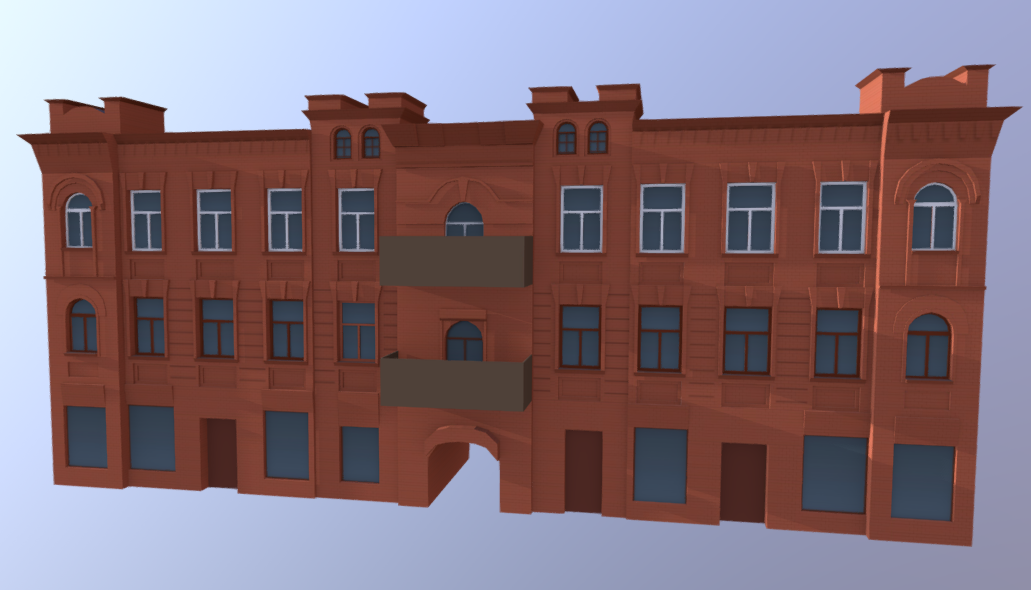
\includegraphics[width=11cm]{src/model_2}} \\
    \hline
    \textbf{Критерий} & \textbf{Балл/ Max.балл} & \textbf{Комментарии} \\
    \hline
    Количество полигонов < 3k.& 0.9/0.9 & Количество полигонов - 2 773, соответствует допустимому диапазону.\\
    \hline 
    Детализация. & 0.7/0.7 & Модель не является примитивом, отдельные части не перегружены лишними деталями, детализация не влияет на критерий количества полигонов. \\
    \hline
    Сходство с реальным объектом. & 0.7/0.7 & Объект можно легко опознать при сравнении с оригиналом - сохранены общие пропорции здания, характерные детали и количественный фактор (окна, двери и т.п.) \\
    \hline
    UV-развертка. & 0.6/0.6 & Развертка присутствует. Вес развертки правильный (окрашена в равномерный синий цвет без ярких зеленых или желтых зон). 
    
    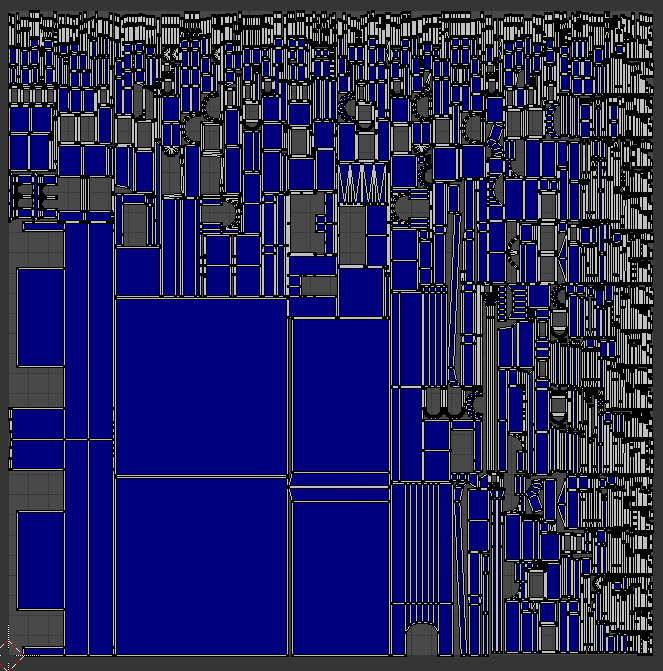
\includegraphics[width=7cm]{src/uv_2} \\
    \hline\\
    Наличие текстур. & 2.0/2.0 & Текстура присутствует (+ дополнительная текстура для ambient occlusion), все текстурные элементы запечены на одну текстуру.

    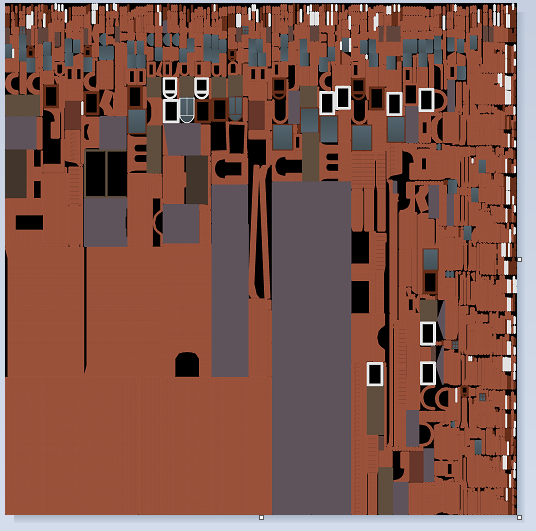
\includegraphics[width=7cm]{src/tec_3}\\
    & & 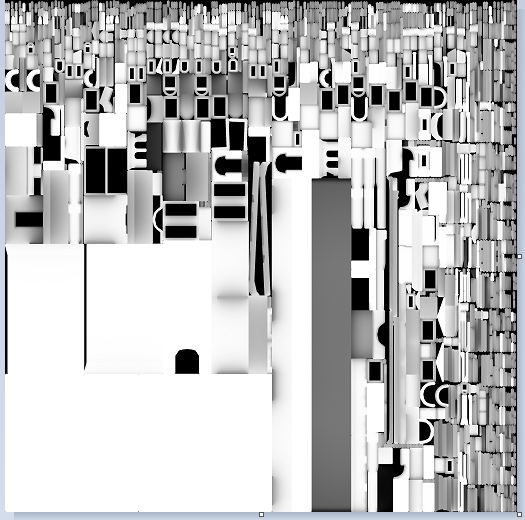
\includegraphics[width=7cm]{src/tec_4}\\
    \hline
    Отсутствие перевернутых нормалей. & 0.45/0.45 & Оси нормалей отображаются верно, направлены из объекта, а не вовнутрь. Нет затемненных участков меша или участков объекта без отображаемых текстур (свидетельство перевернутых нормалей).
    
    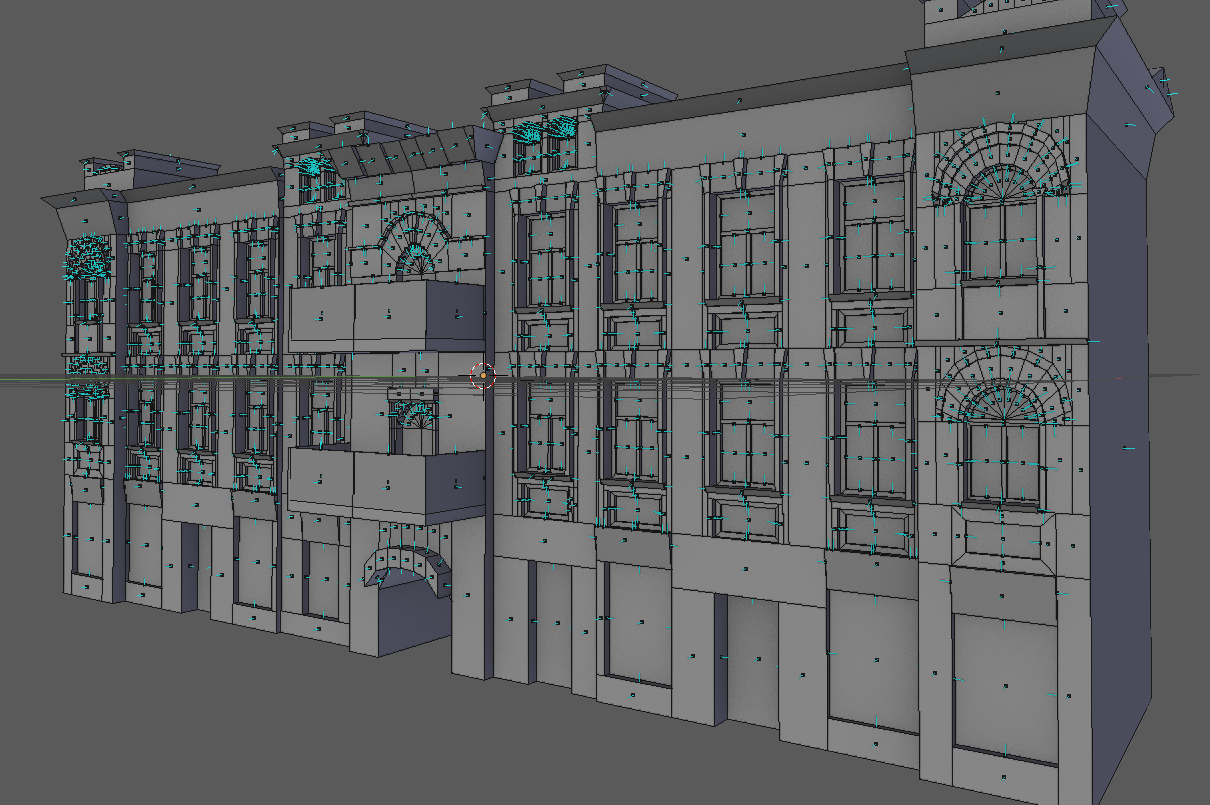
\includegraphics[width=7cm]{src/norm_3}\\
    & & 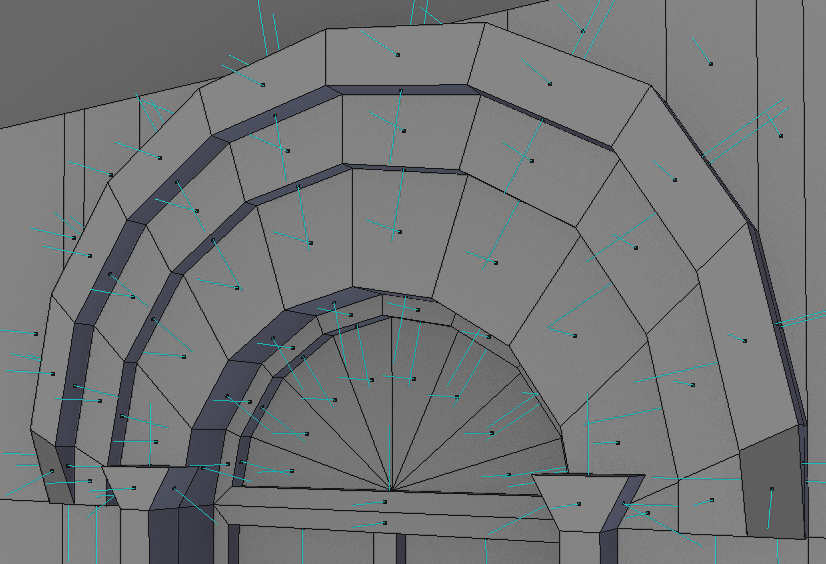
\includegraphics[width=7cm]{src/norm_4}\\
    \hline
    Отсутствие неправильных полигонов. & 0.6/0.6 & Все полигоны имеют форму четырехугольника или треугольника, нет полигонов с большим количеством углов. \\
    \hline
    \multicolumn{3}{|c|}{\textbf{Итого за модель: 5.95}}\\
    \hline
\end{longtable}

\begin{center}
    \textbf{Модель №3}
\end{center}

\begin{longtable}{|p{4cm}|p{2.5cm}|p{7.5cm}|}
    \hline
    \multicolumn{3}{|c|}{\textbf{Оригинальное здание} } \\
    \hline
    \multicolumn{3}{|c|}{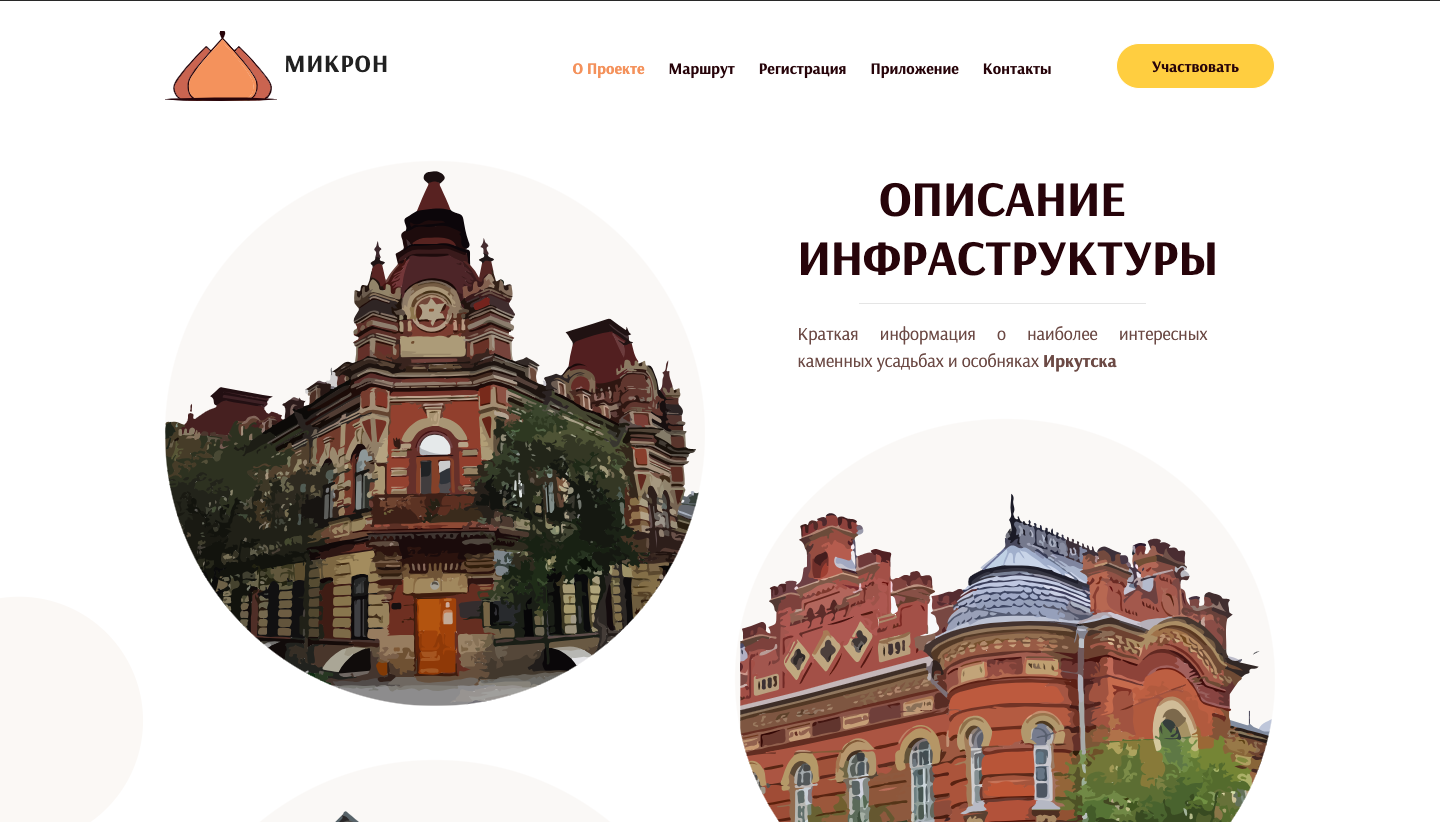
\includegraphics[width=11cm]{2}} \\
    \hline
    \multicolumn{3}{|c|}{\textbf{Модель}} \\
    \hline
    \multicolumn{3}{|c|}{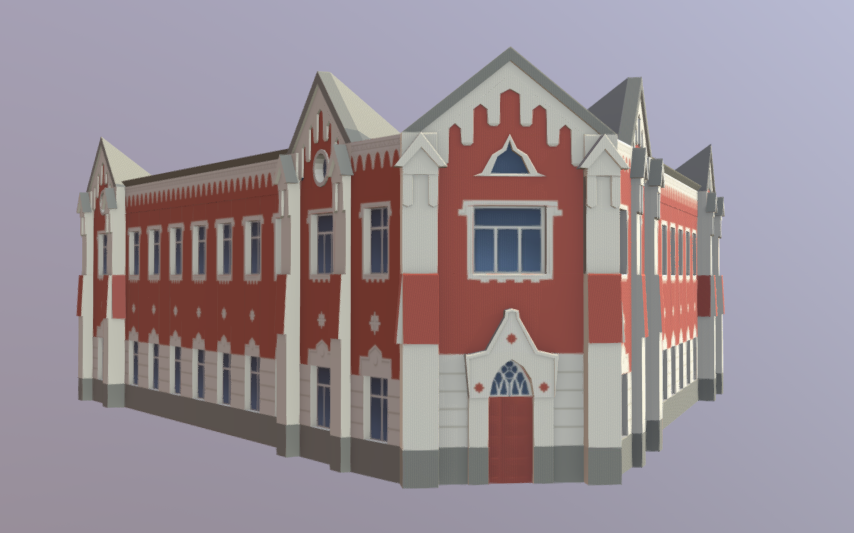
\includegraphics[width=11cm]{src/model_3}} \\
    \hline
    \textbf{Критерий} & \textbf{Балл/ Max.балл} & \textbf{Комментарии} \\
    \hline
    Количество полигонов < 3k. & 0.9/0.9 & Количество полигонов - 1 803, соответствует допустимому диапазону. \\
    \hline
    Детализация. & 0.7/0.7 & Модель не является примитивом, отдельные части не перегружены лишними деталями, детализация не влияет на критерий количества полигонов. \\
    \hline
    Сходство с реальным объектом. & 0.7/0.7 & Объект можно легко опознать при сравнении с оригиналом - сохранены общие пропорции здания, характерные детали и количественный фактор (окна, двери и т.п.) \\
    \hline
    UV-развертка. & 0.6/0.6 & Развертка присутствует. Вес развертки правильный (окрашена в равномерный синий цвет без ярких зеленых или желтых зон). 
    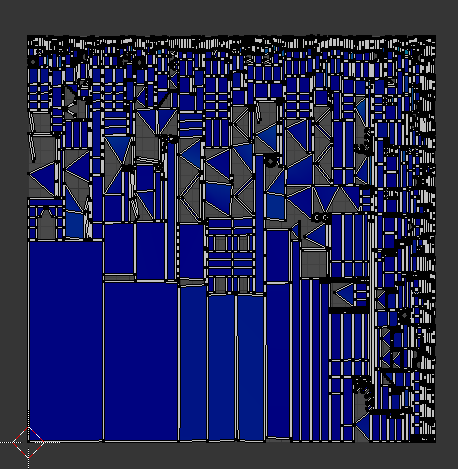
\includegraphics[width=7cm]{src/uv_3}\\
    \hline
    Наличие текстур. & 2.0/2.0 & Текстура присутствует (+ дополнительная текстура для ambient occlusion), все текстурные элементы запечены на одну текстуру.

    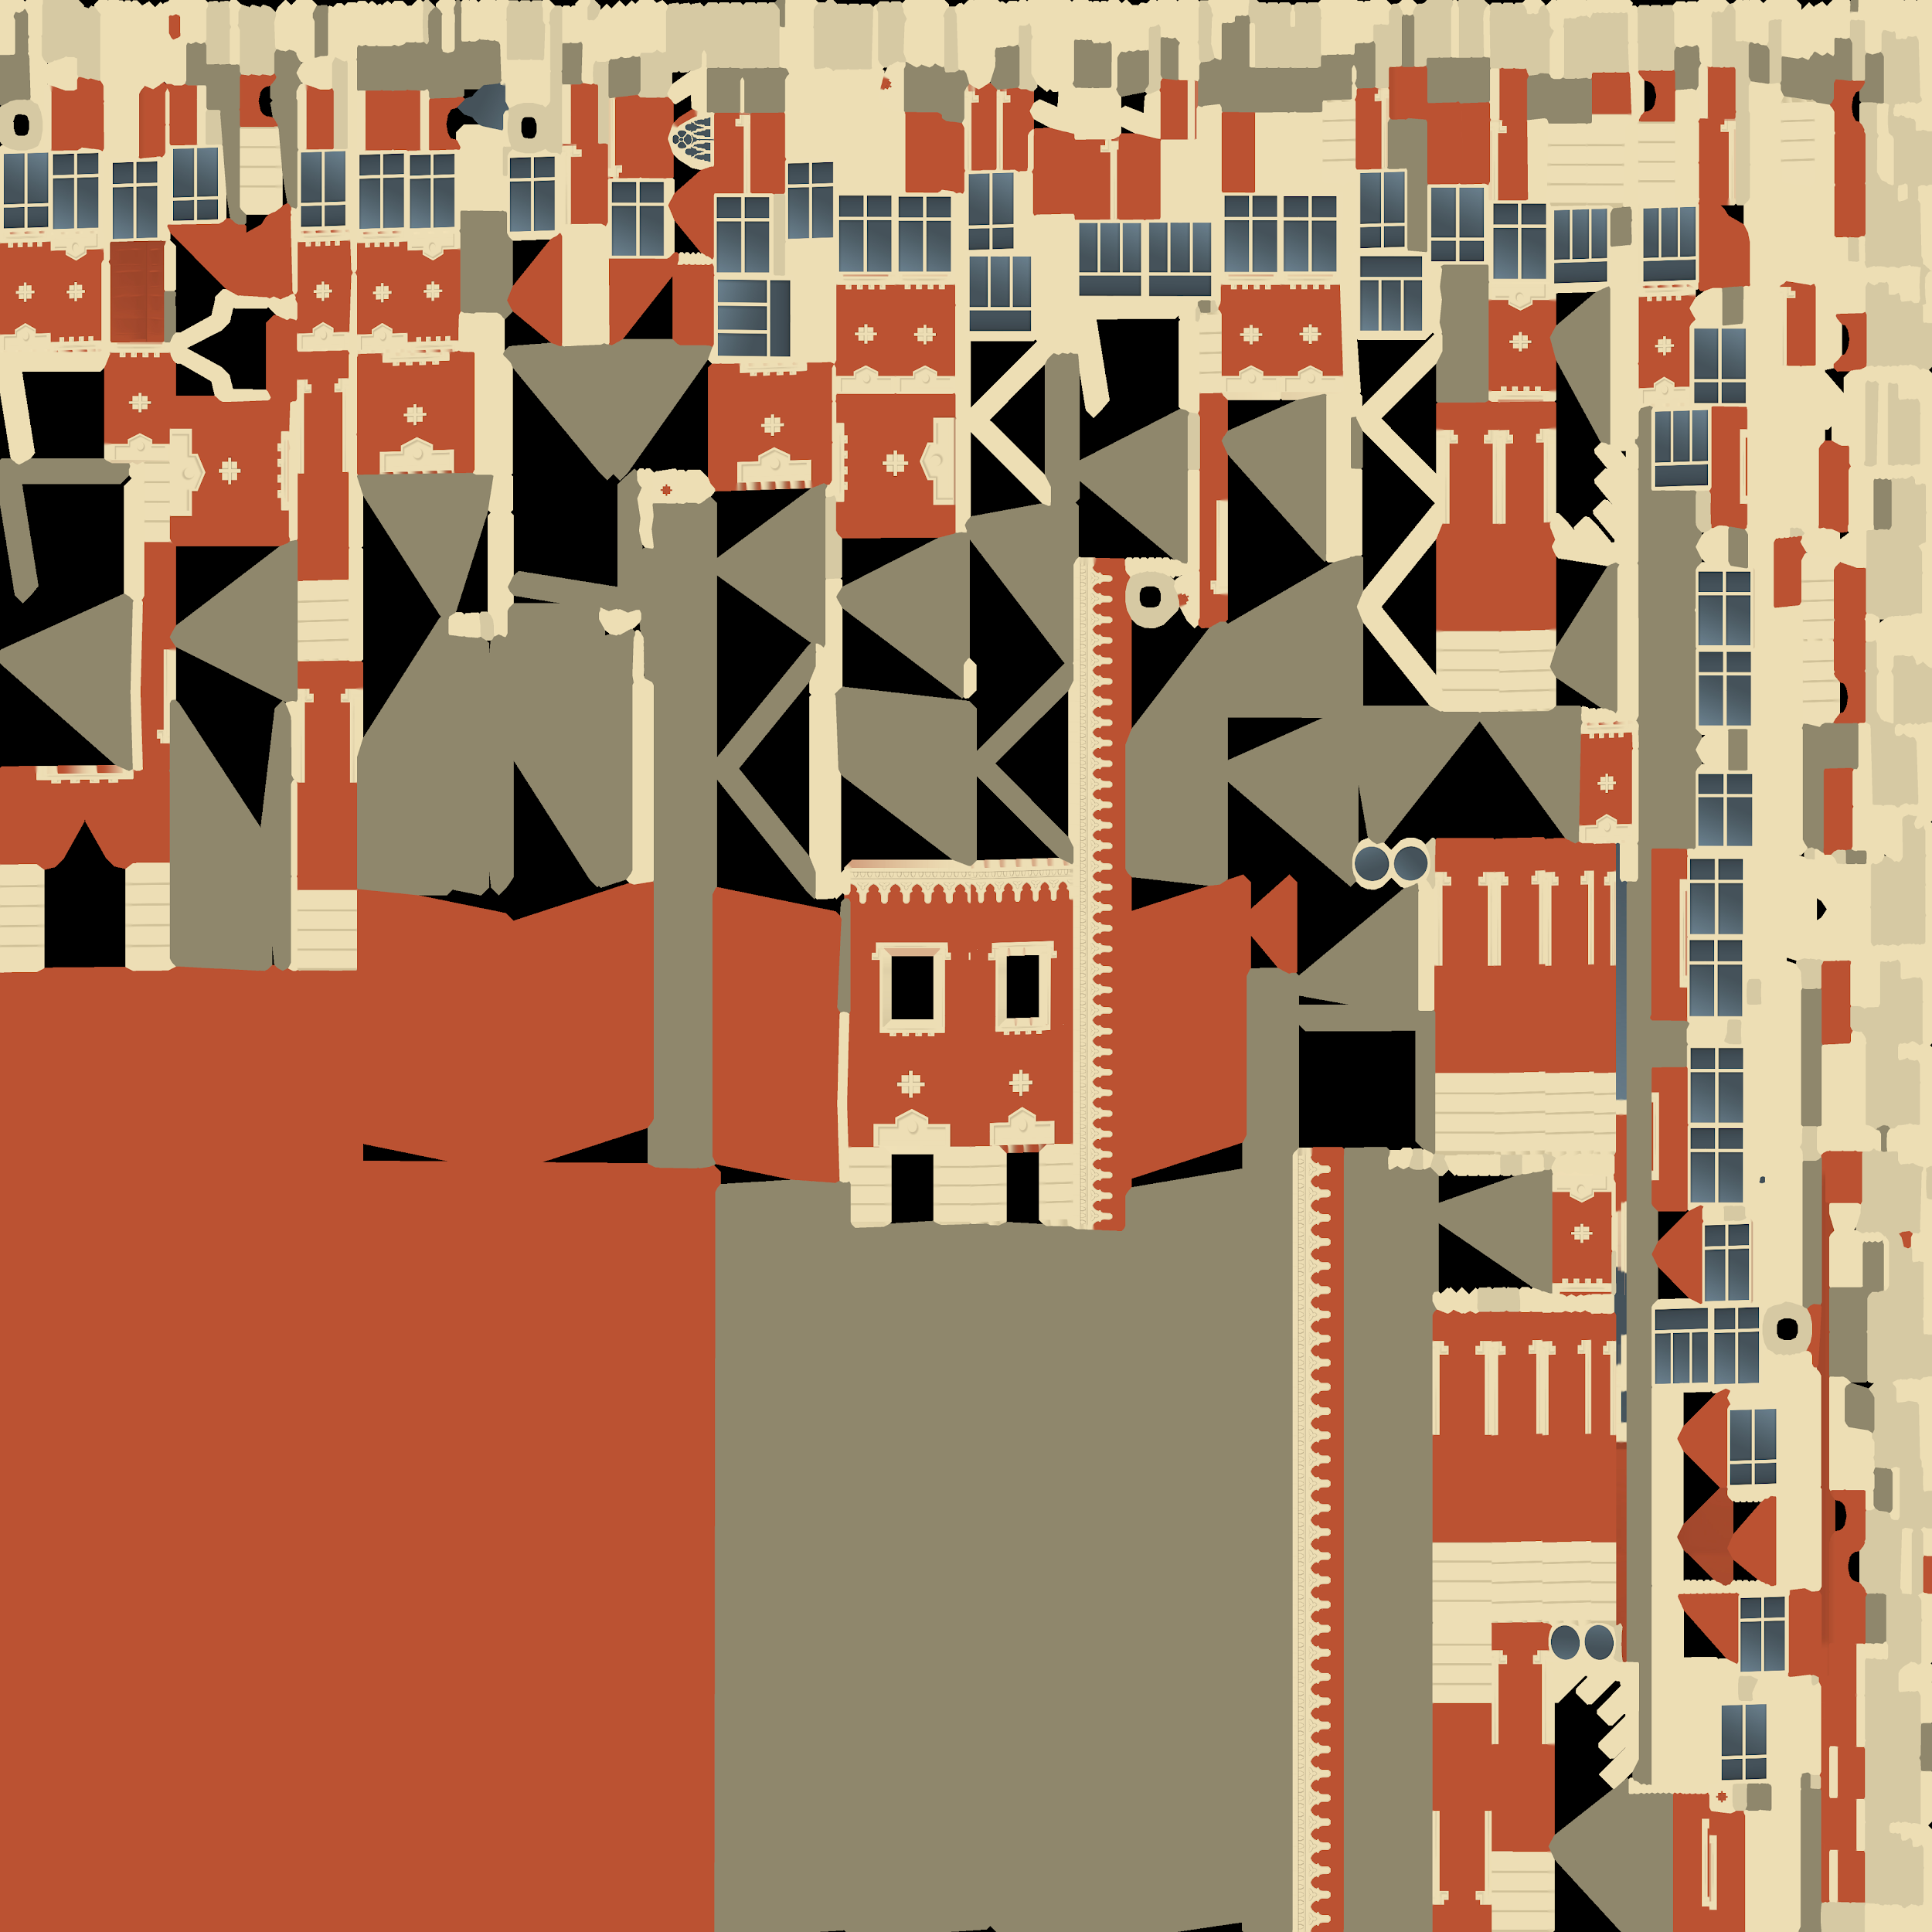
\includegraphics[width=7cm]{src/tec_5}\\
    & & 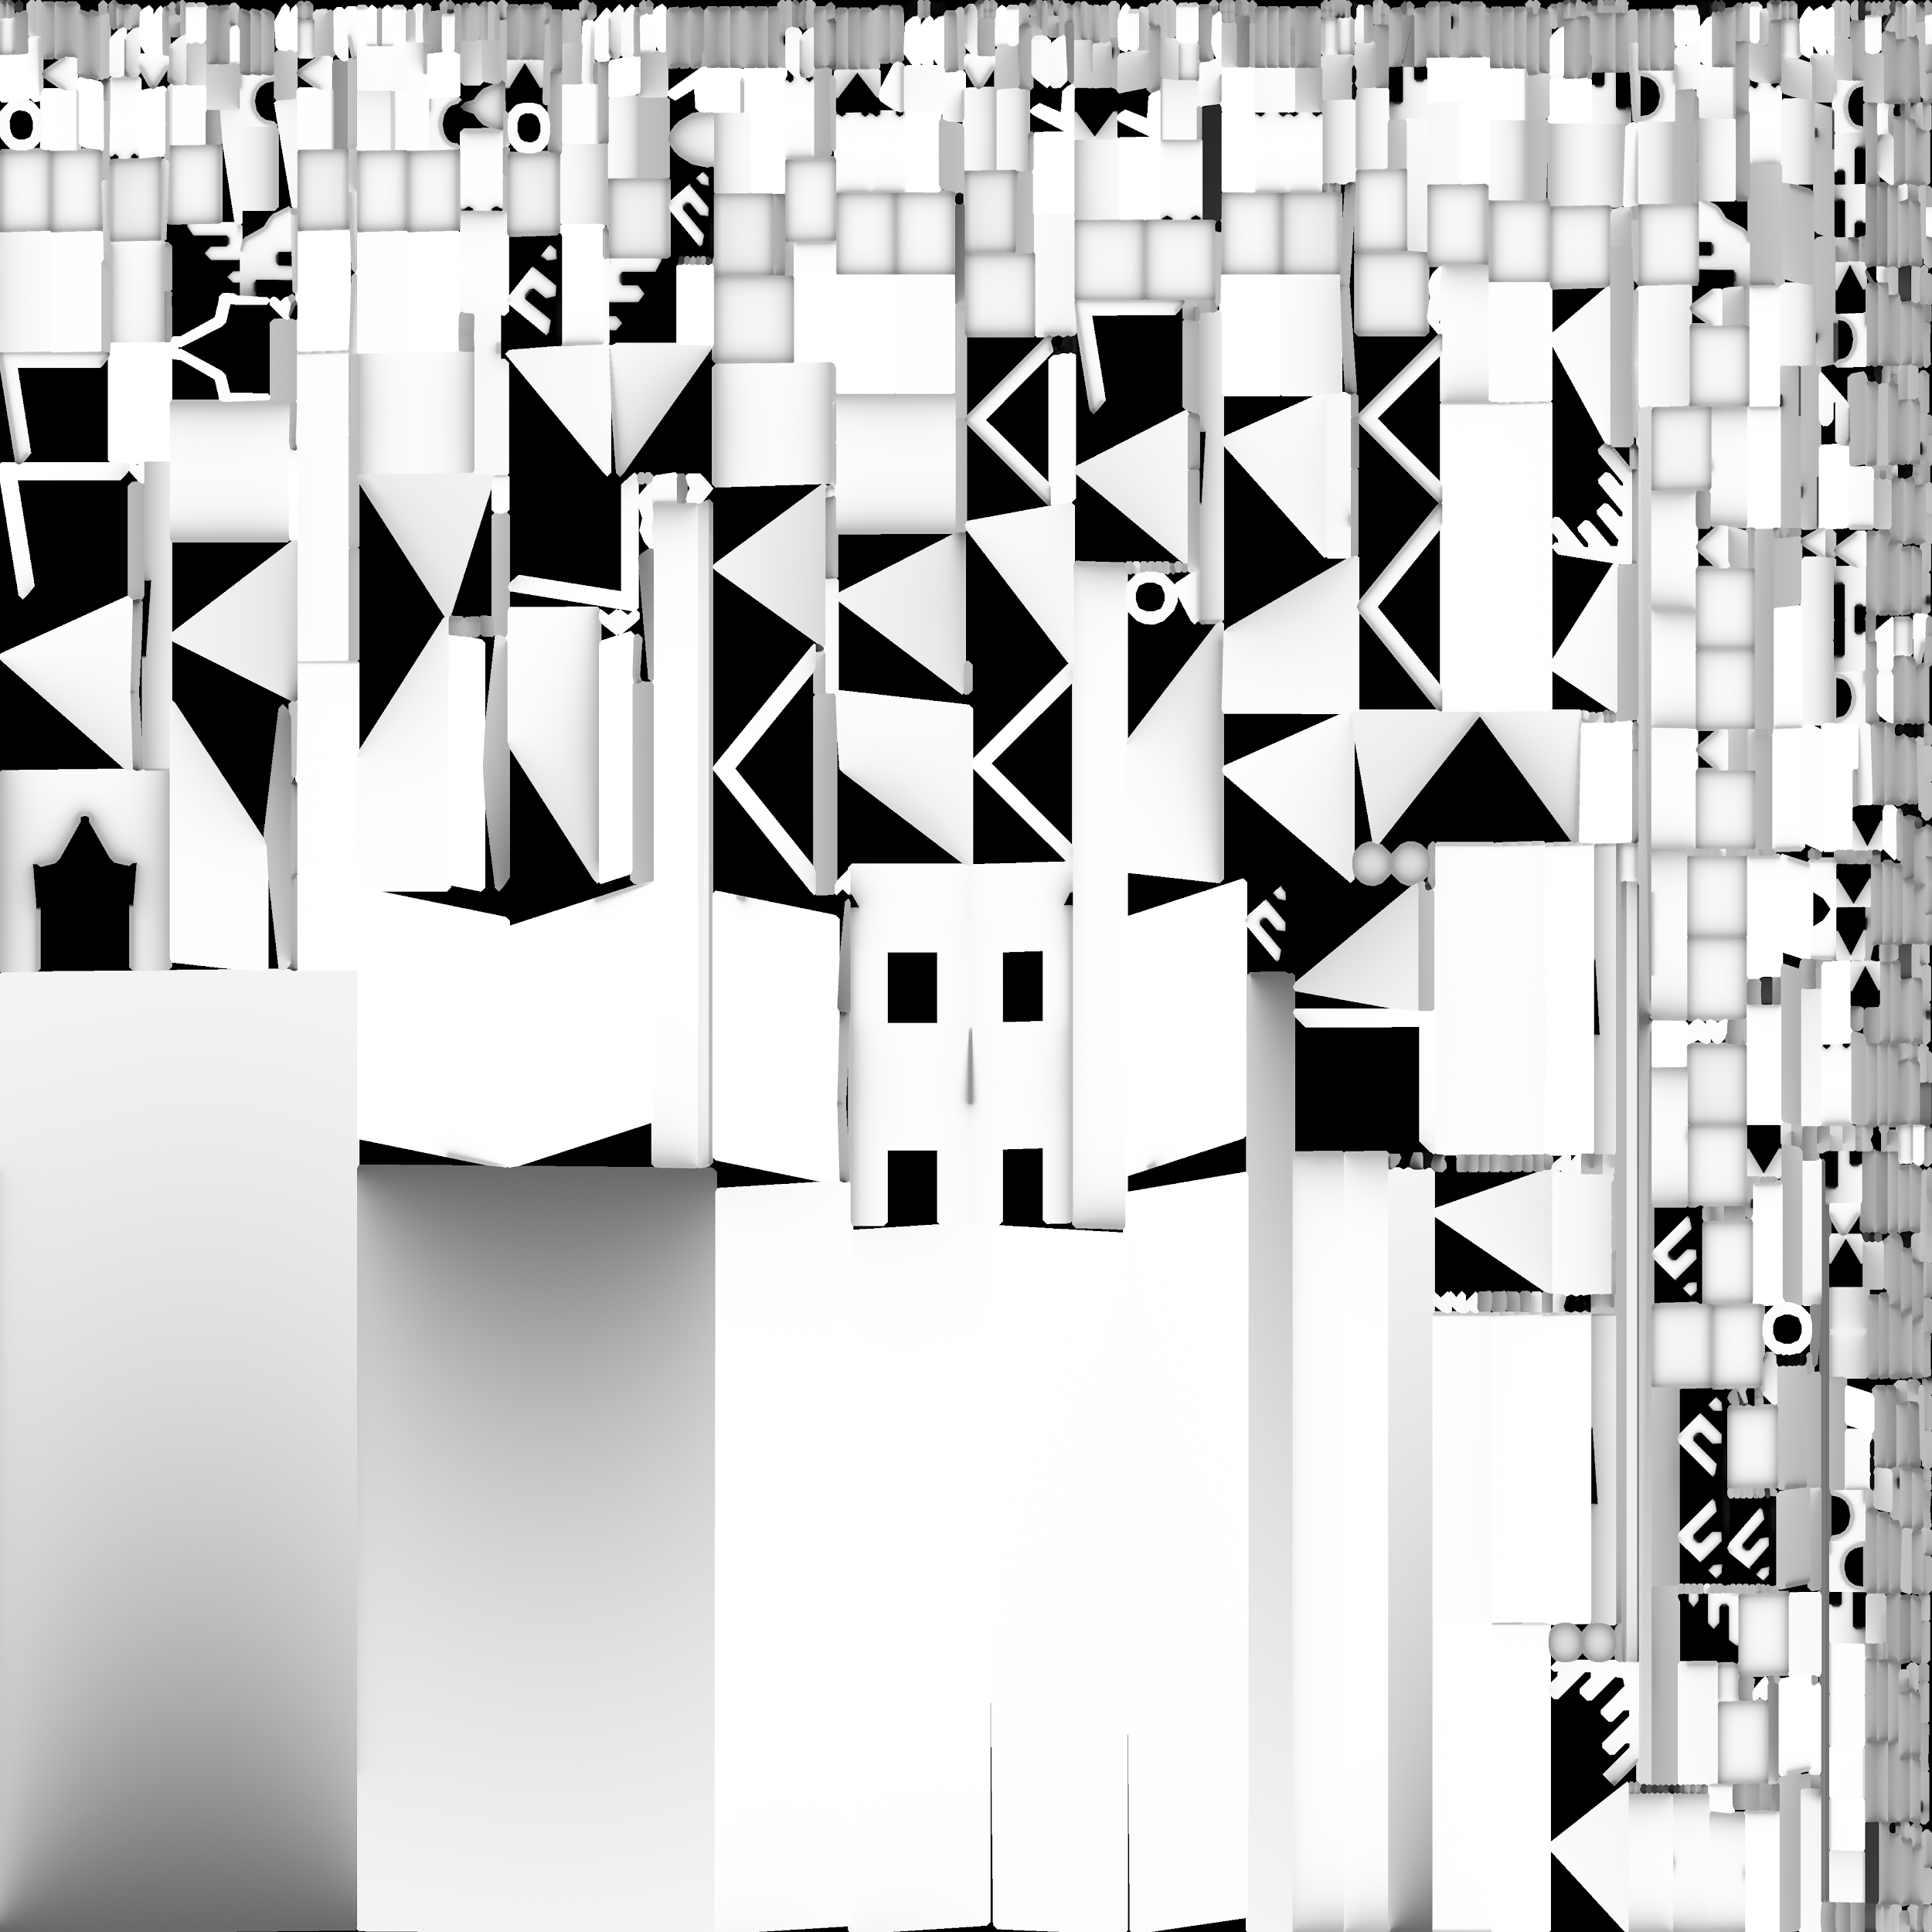
\includegraphics[width=7cm]{src/tec_6}\\
    \hline

    Отсутствие перевернутых нормалей. & 0.45/0.45 & Оси нормалей отображаются верно, направлены из объекта, а не вовнутрь. Нет затемненных участков меша или участков объекта без отображаемых текстур (свидетельство перевернутых нормалей).

    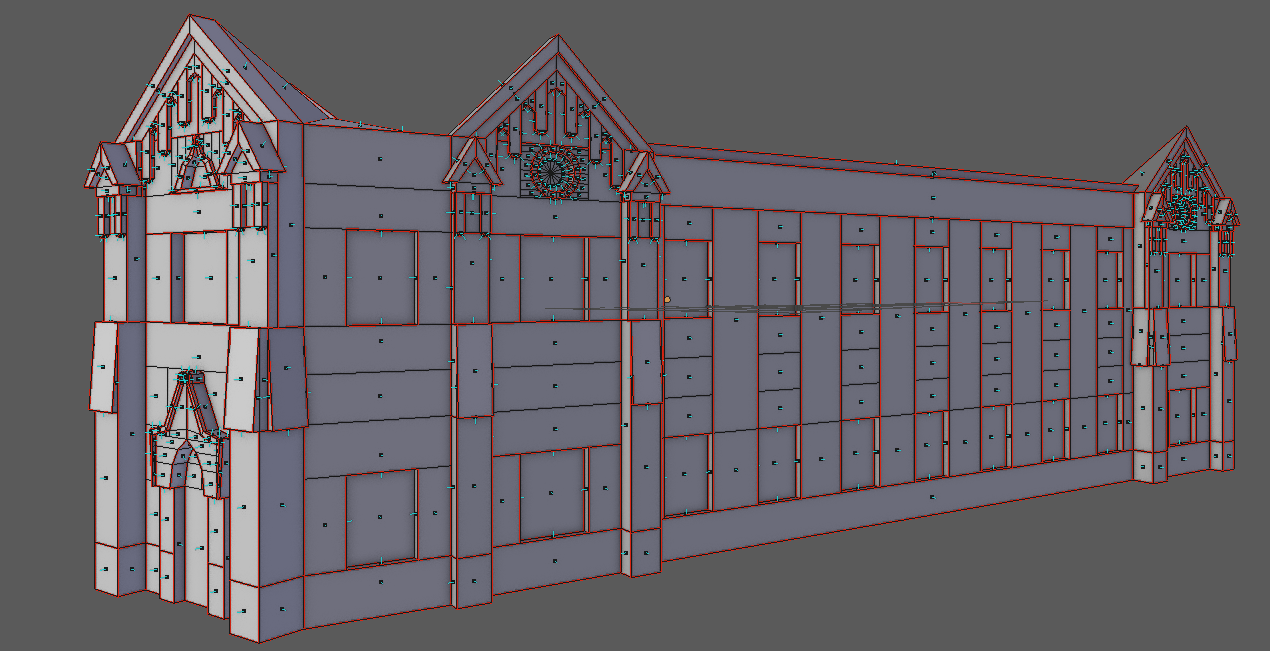
\includegraphics[width=7cm]{src/norm_5}\\
    & & 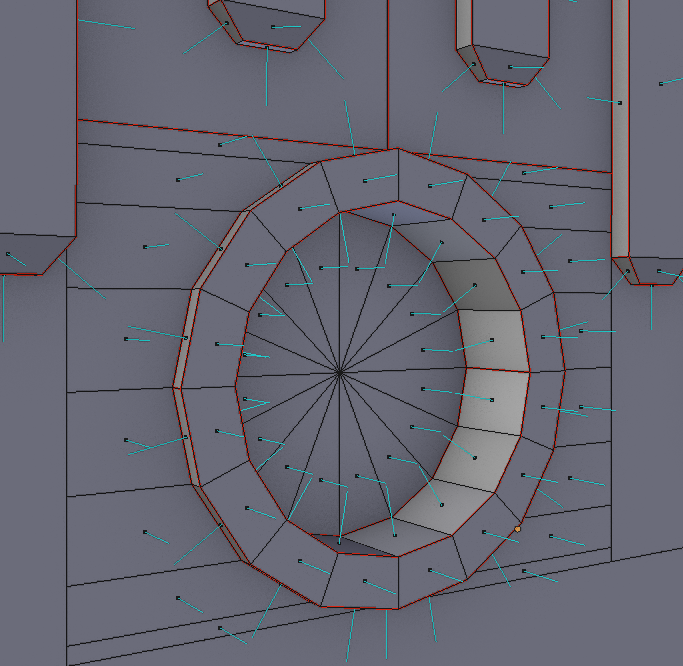
\includegraphics[width=7cm]{src/norm_6} \\
    \hline
    Отсутствие неправильных полигонов. & 0.6/0.6 & Все полигоны имеют форму четырехугольника или треугольника, нет полигонов с большим количеством углов. \\
    \hline
    \multicolumn{3}{|c|}{\textbf{Итого за модель: 5.95}}\\
    \hline
\end{longtable}

\begin{center}
    \textbf{Модель №4}
\end{center}

\begin{longtable}{|p{4cm}|p{2.5cm}|p{7.5cm}|}
    \hline
    \multicolumn{3}{|c|}{\textbf{Оригинальное здание} } \\
    \hline
    \multicolumn{3}{|c|}{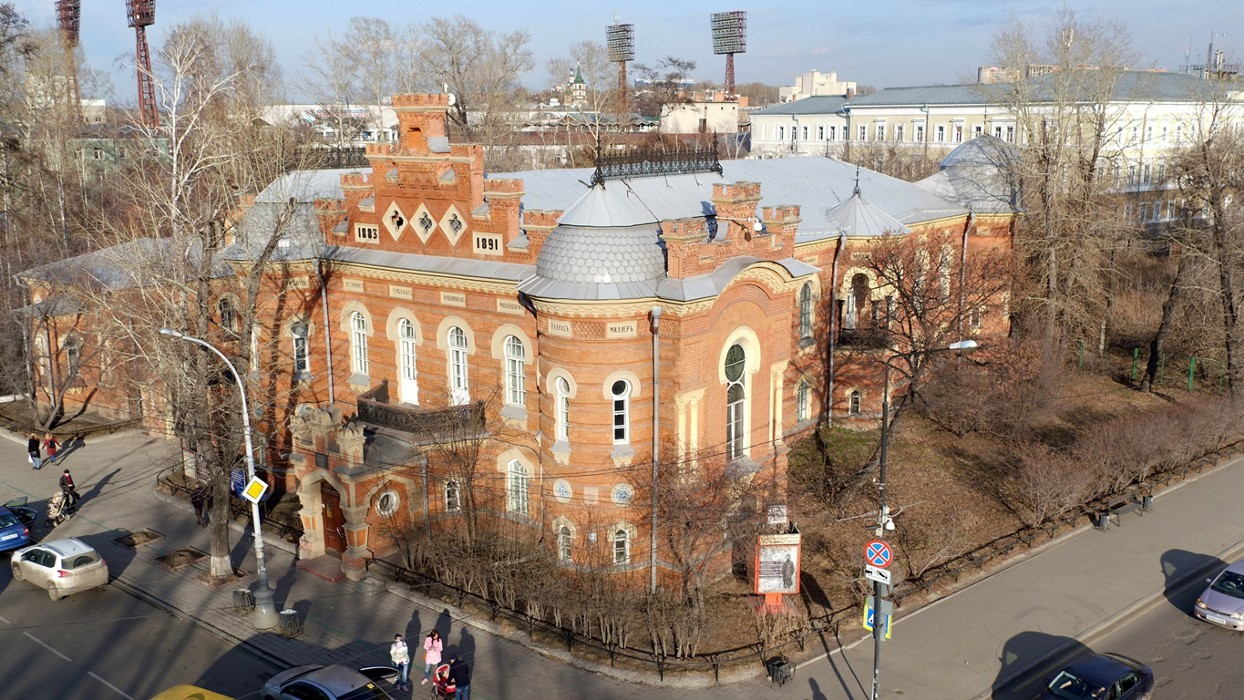
\includegraphics[width=11cm]{src/build_4}} \\
    \hline
    \multicolumn{3}{|c|}{\textbf{Модель}} \\
    \hline
    \multicolumn{3}{|c|}{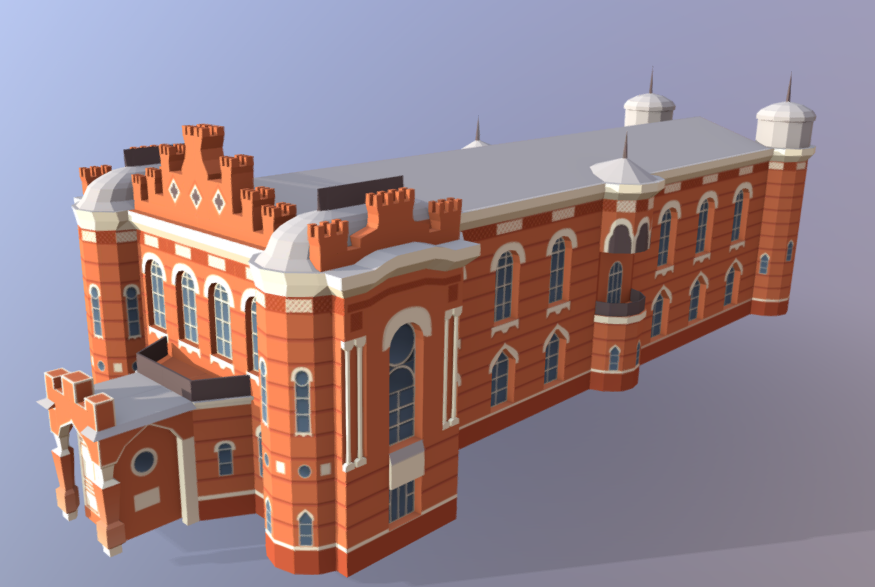
\includegraphics[width=11cm]{src/model_4}} \\
    \hline
    \textbf{Критерий} & \textbf{Балл/ Max.балл} & \textbf{Комментарии} \\
    \hline
    Количество полигонов < 3k. & 0.9/0.9 & оличество полигонов - 2 983, соответствует допустимому диапазону. \\
    \hline
    Детализация. & 0.7/0.7 & одель не является примитивом, отдельные части не перегружены лишними деталями, детализация не влияет на критерий количества полигонов. \\
    \hline
    Сходство с реальным объектом. & 0.7/0.7 & бъект можно легко опознать при сравнении с оригиналом - сохранены общие пропорции здания, характерные детали и количественный фактор (окна, двери и т.п.) \\
    \hline
    UV-развертка. & 0.6/0.6 & азвертка присутствует. Вес развертки правильный (окрашена в равномерный синий цвет без ярких зеленых или желтых зон). 
    
    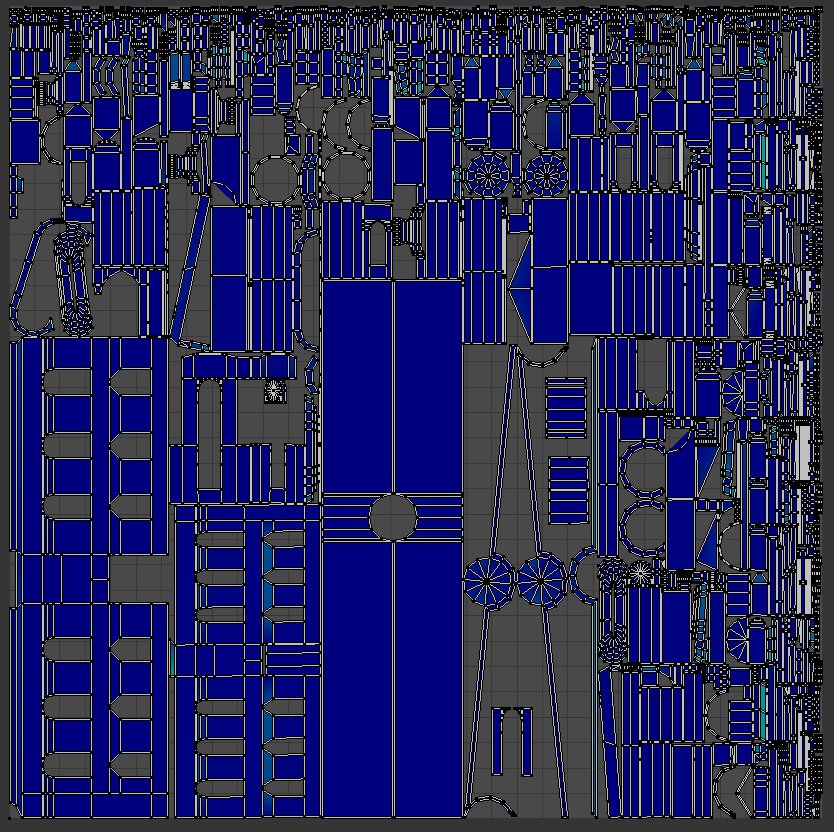
\includegraphics[width=7cm]{src/uv_4}
    \\
    \hline
    Наличие текстур. & 2.0/2.0 & Текстура присутствует (+ дополнительная текстура для ambient occlusion), все текстурные элементы запечены на одну текстуру.

    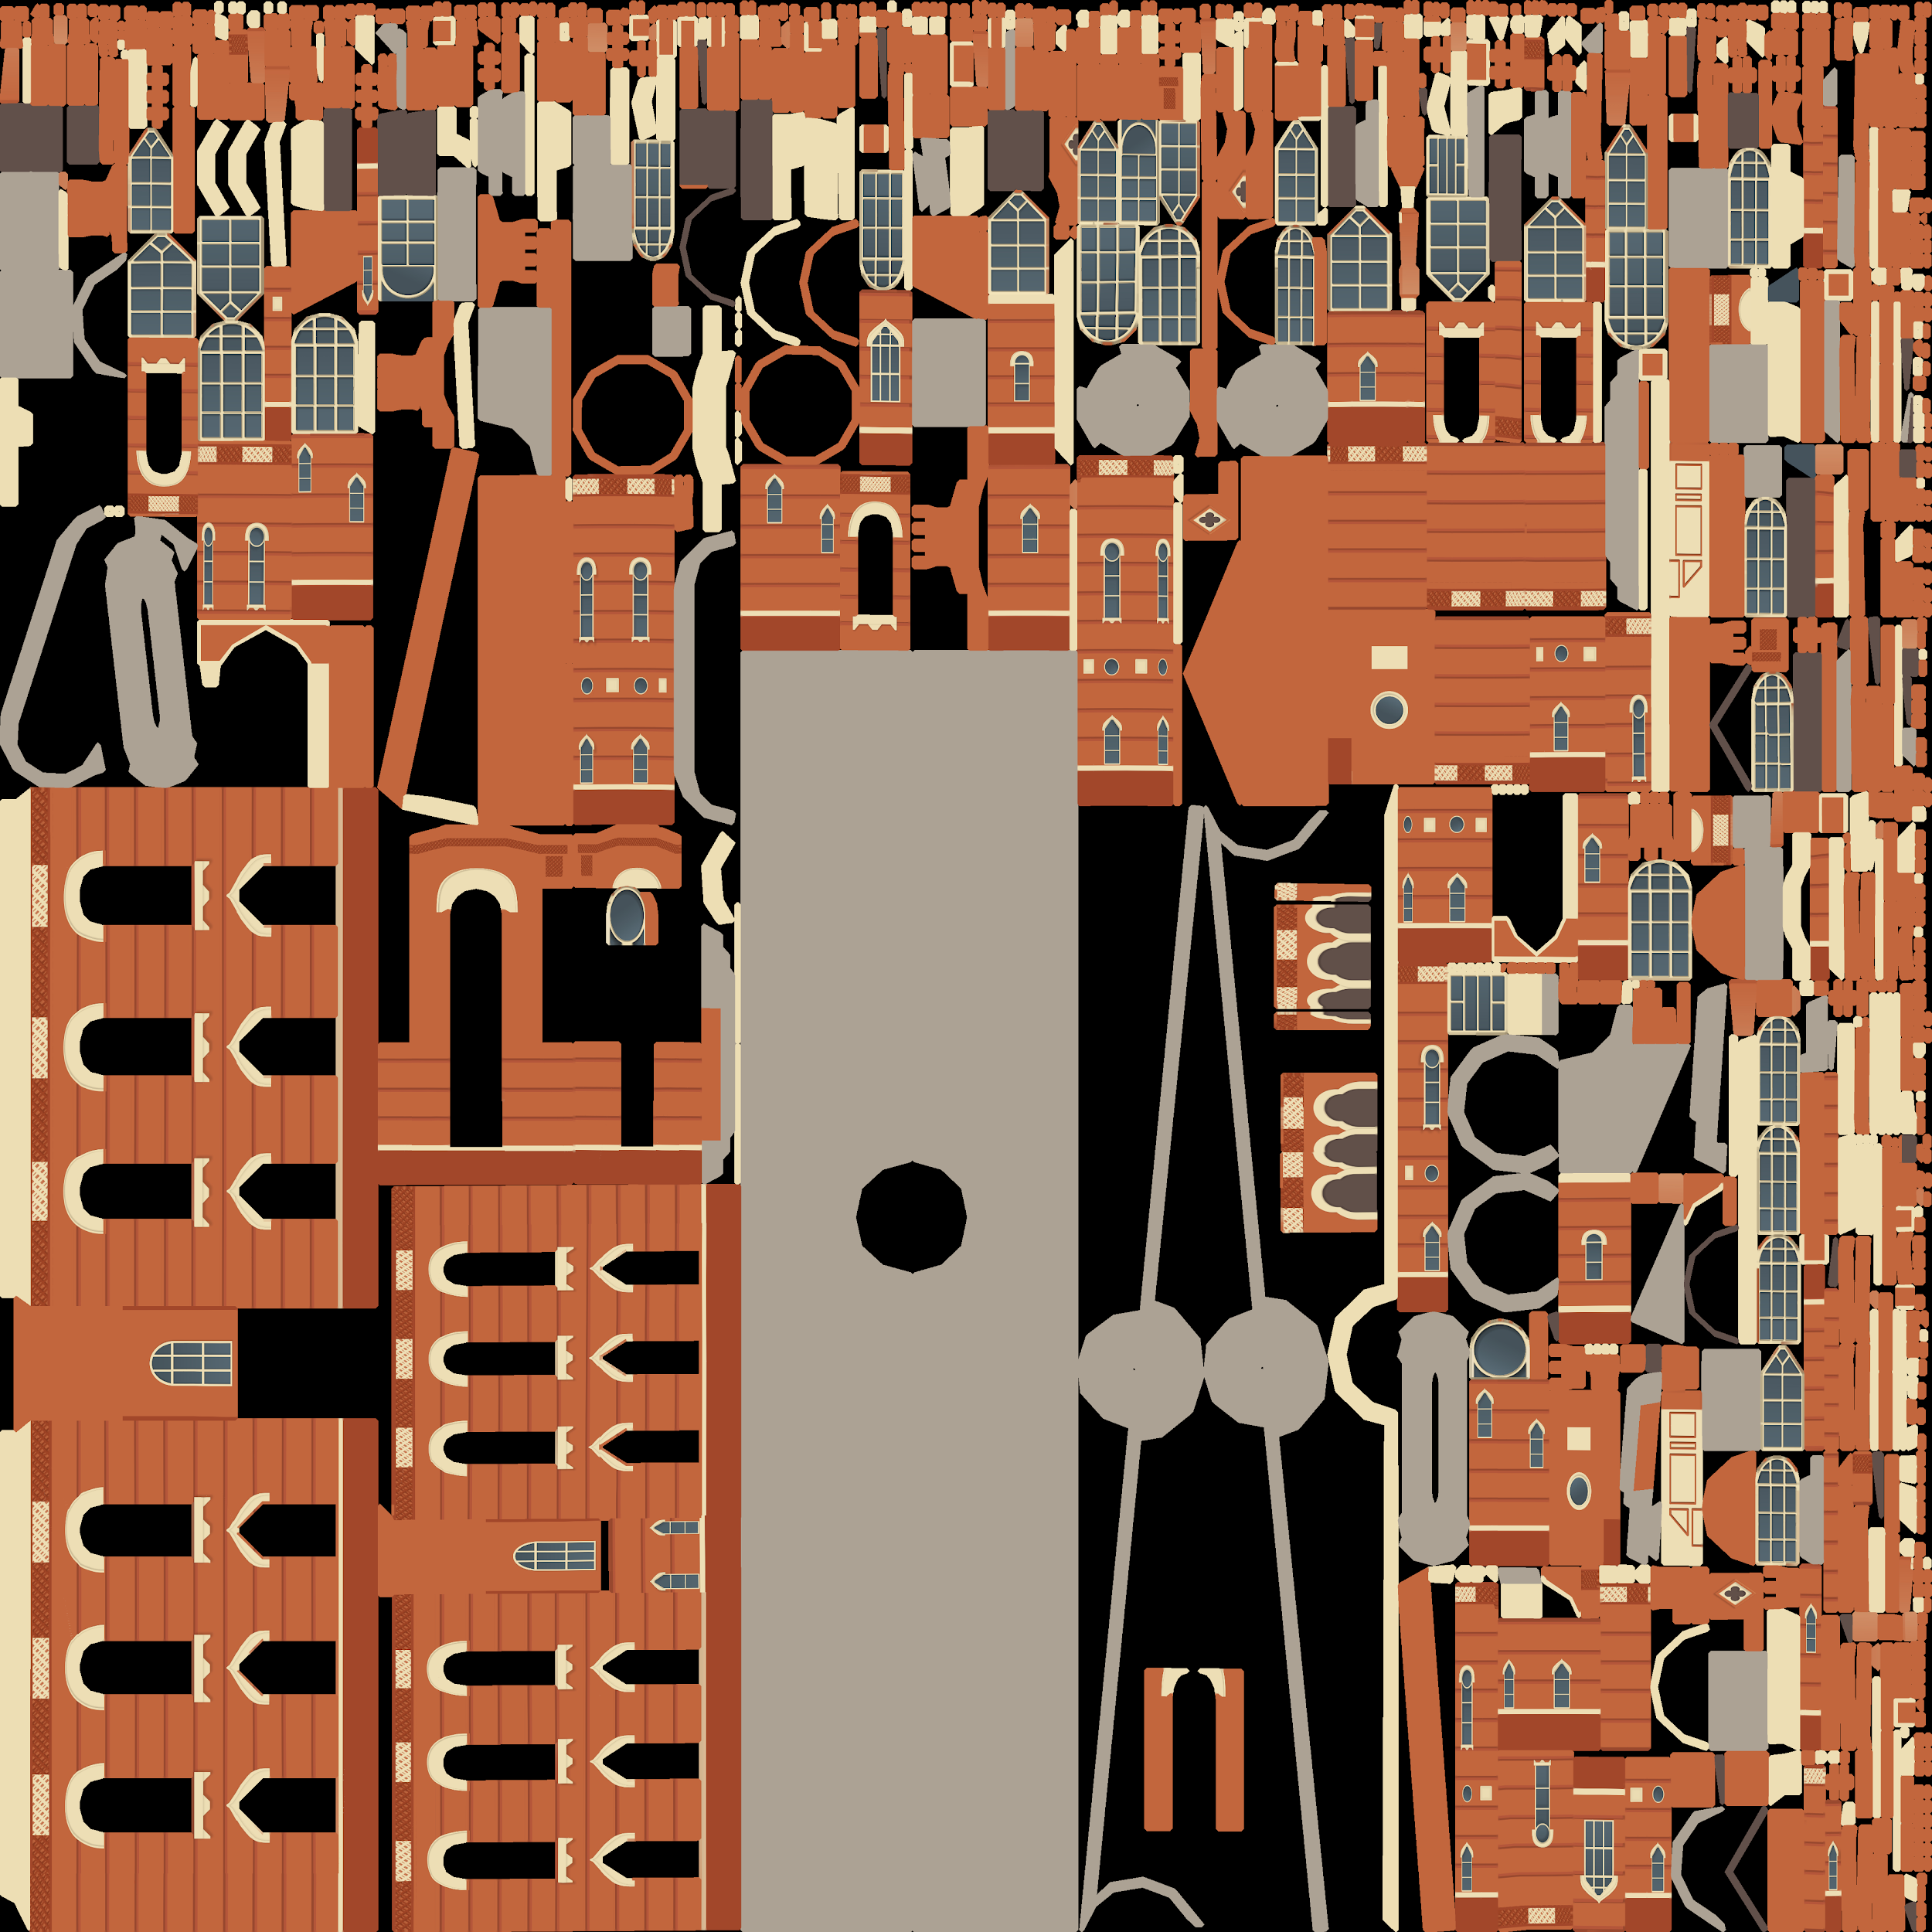
\includegraphics[width=7cm]{src/tec_7}\\
    & & 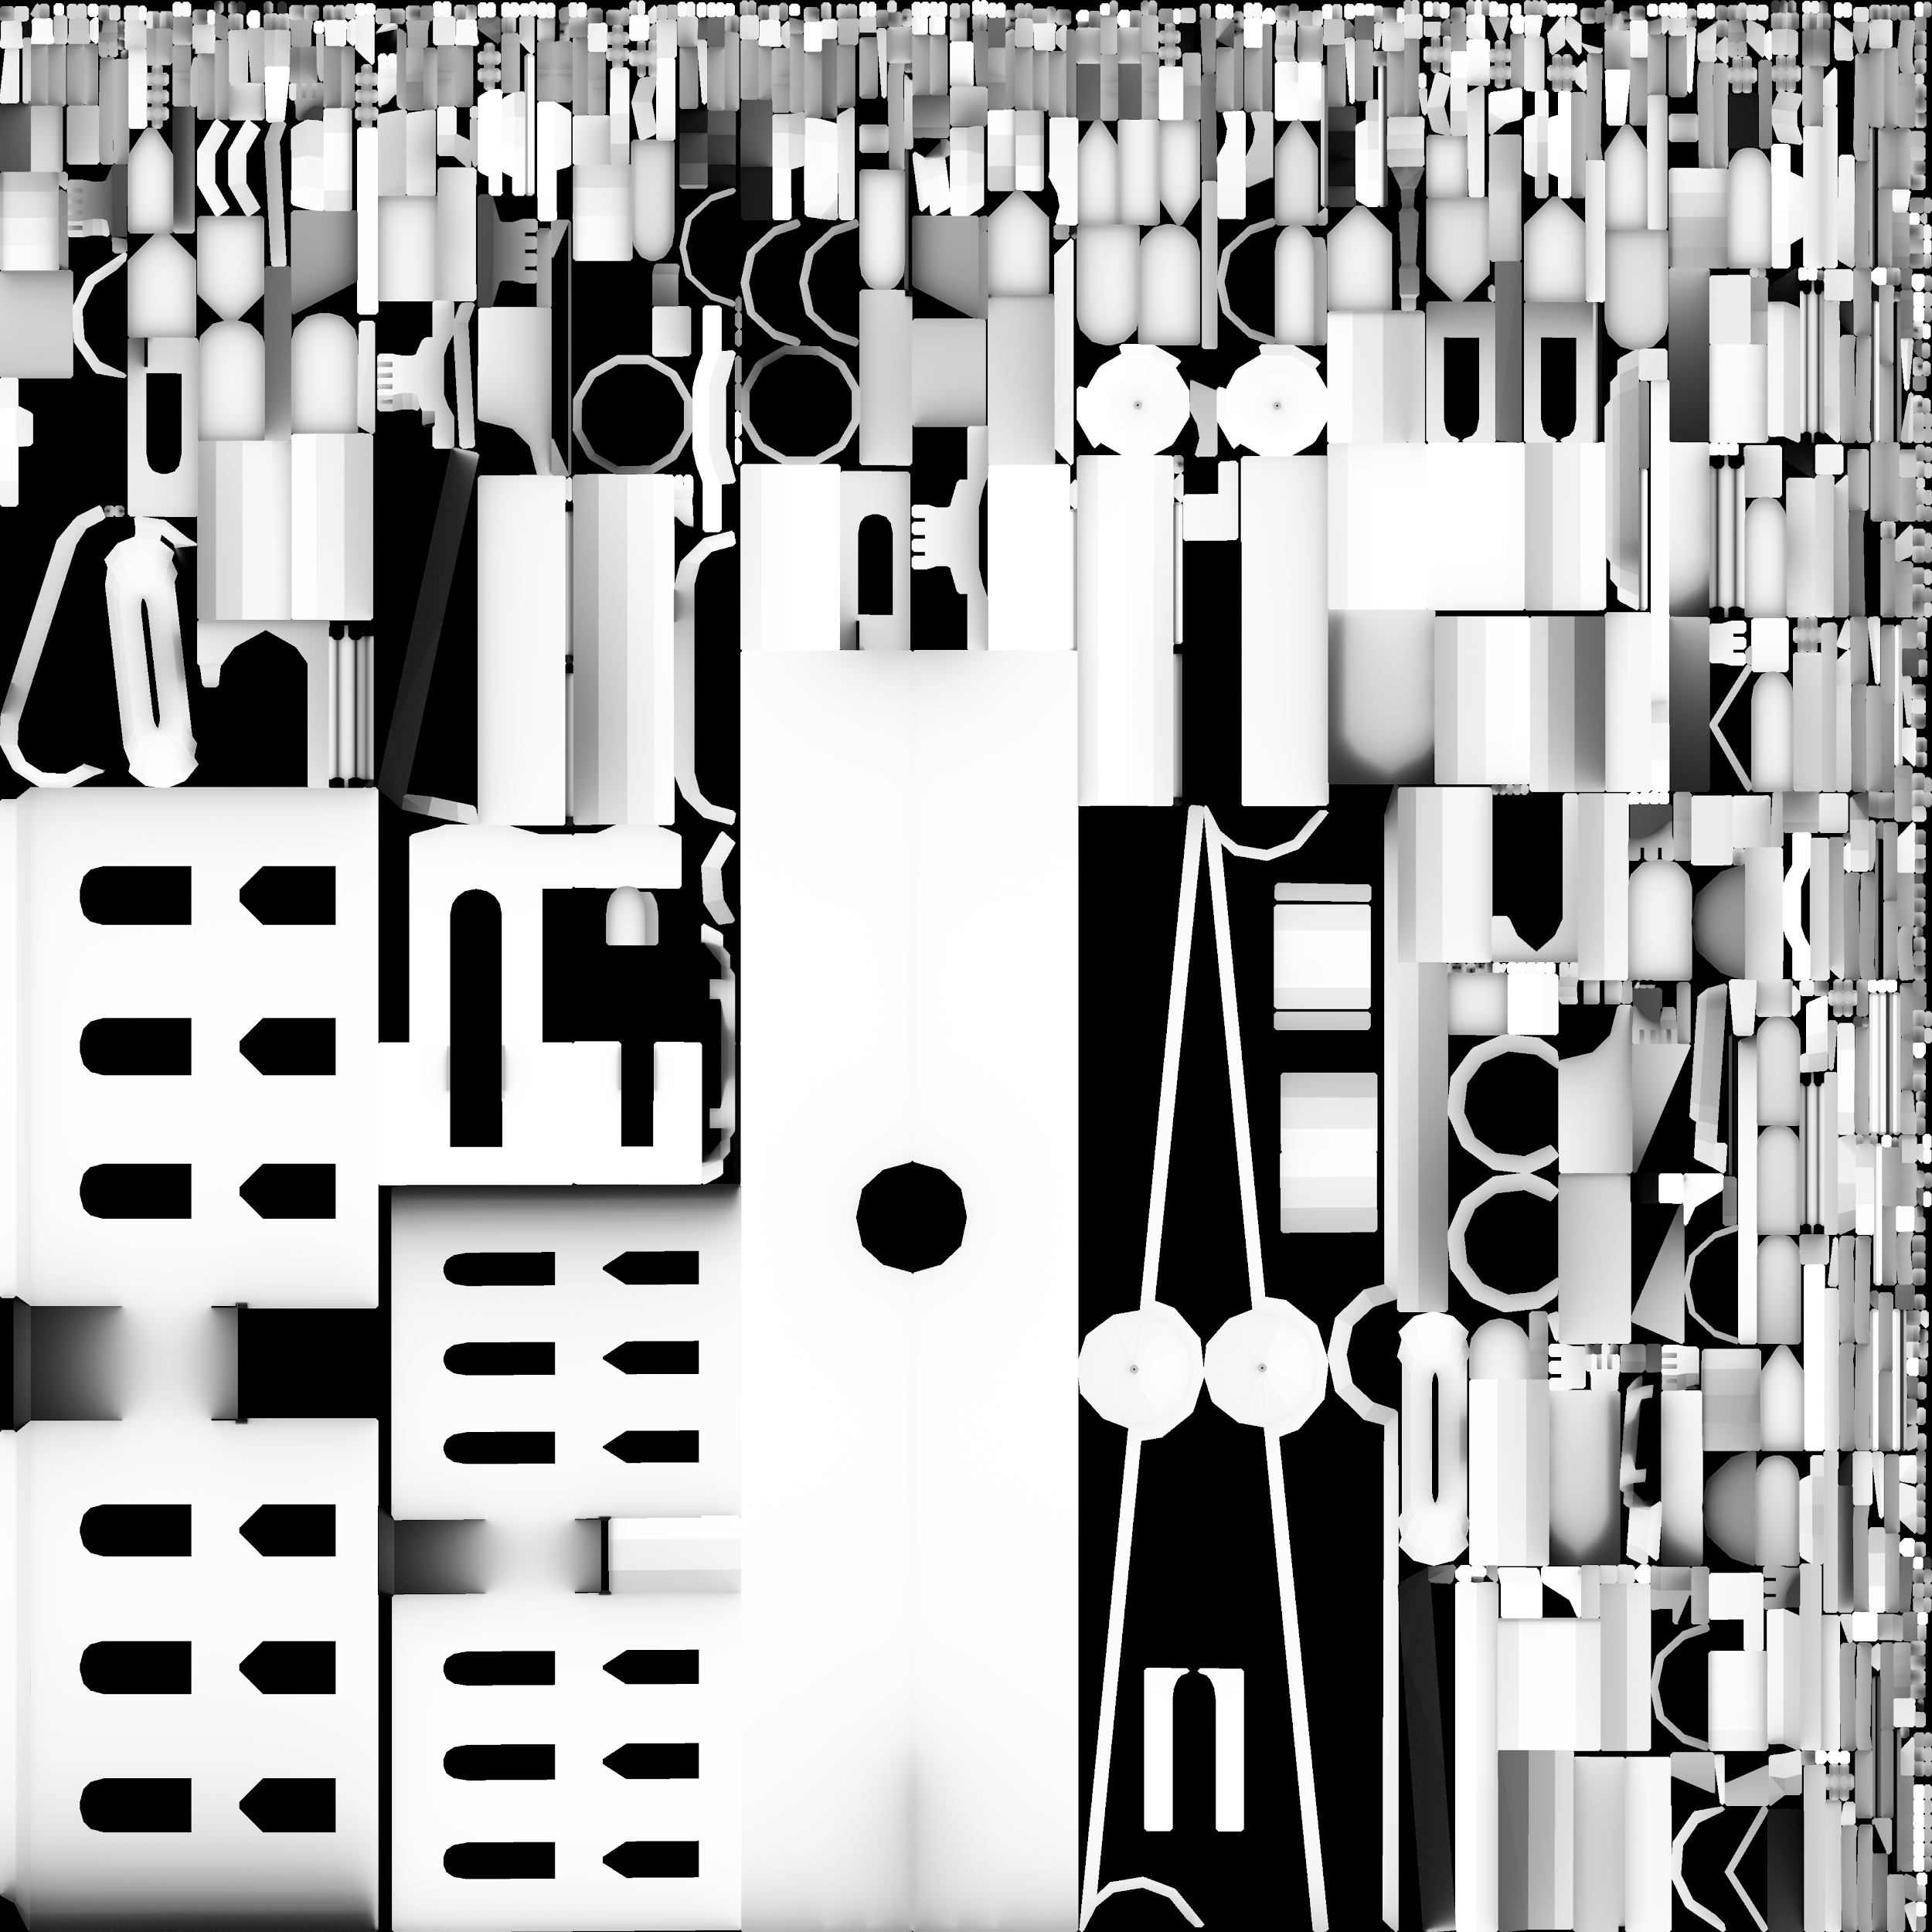
\includegraphics[width=7cm]{src/tec_8} \\
    \hline
    Отсутствие перевернутых нормалей. & 0.45/0.45 & Оси нормалей отображаются верно, направлены из объекта, а не вовнутрь. Нет затемненных участков меша или участков объекта без отображаемых текстур (свидетельство перевернутых нормалей).

    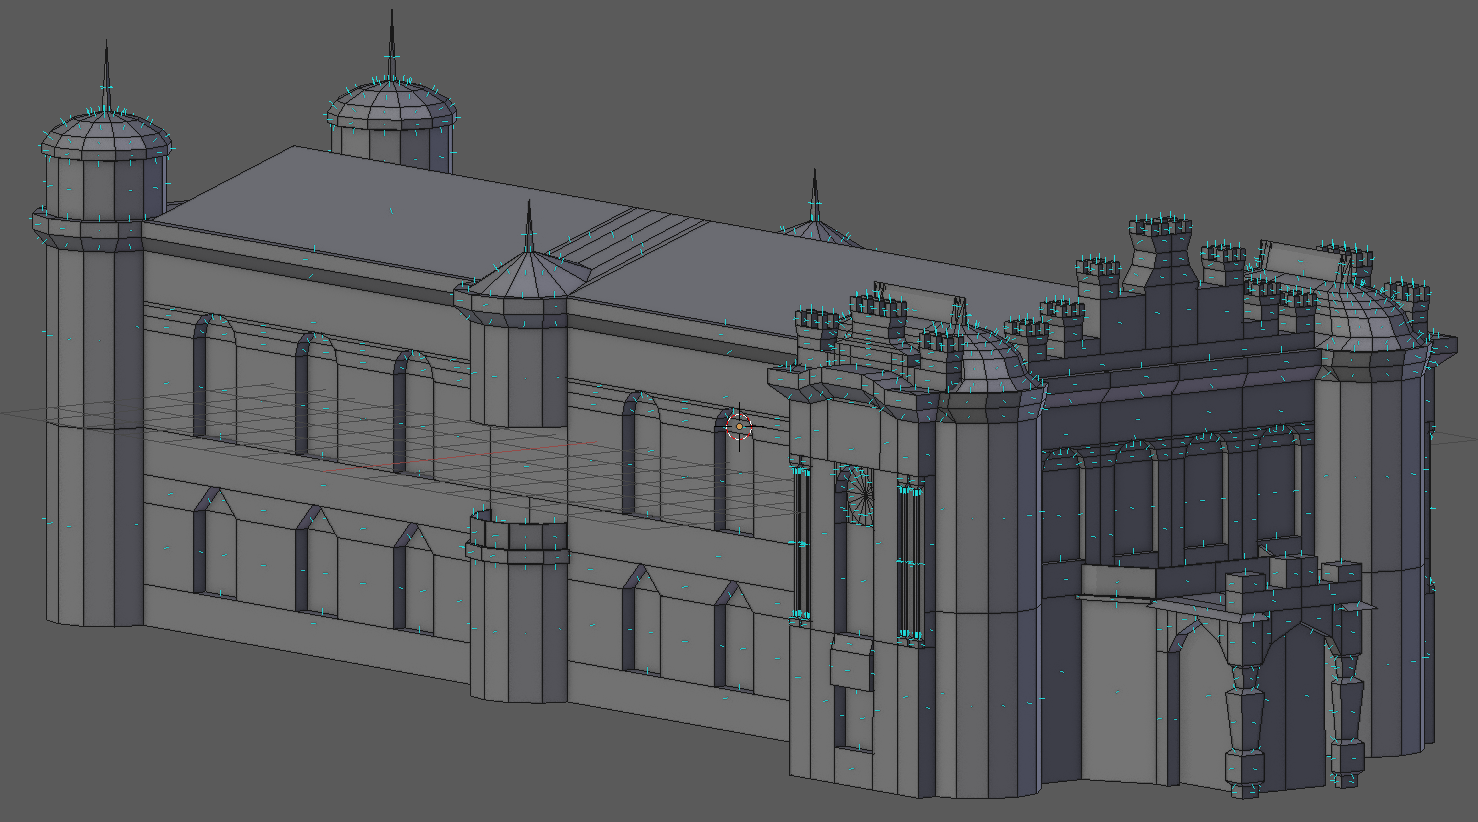
\includegraphics[width=7cm]{src/norm_7}\\
    & & 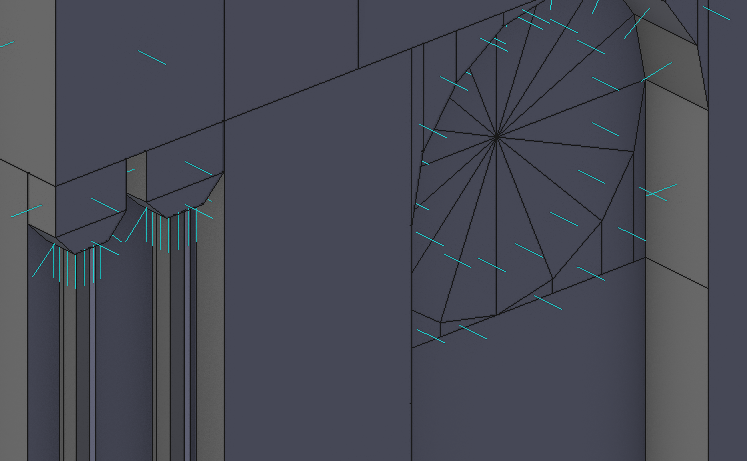
\includegraphics[width=7cm]{src/norm_8} \\
    \hline
    Отсутствие неправильных полигонов. & 0.6/0.6 & Все полигоны имеют форму четырехугольника или треугольника, нет полигонов с большим количеством углов. \\
    \hline 
    \multicolumn{3}{|c|}{\textbf{Итого за модель: 5.95}} \\
    \hline
\end{longtable}

\begin{center}
    \textbf{Модель №5}
\end{center}

\begin{longtable}{|p{4cm}|p{2.5cm}|p{7.5cm}|}
    \hline
    \multicolumn{3}{|c|}{\textbf{Оригинальное здание} } \\
    \hline
    \multicolumn{3}{|c|}{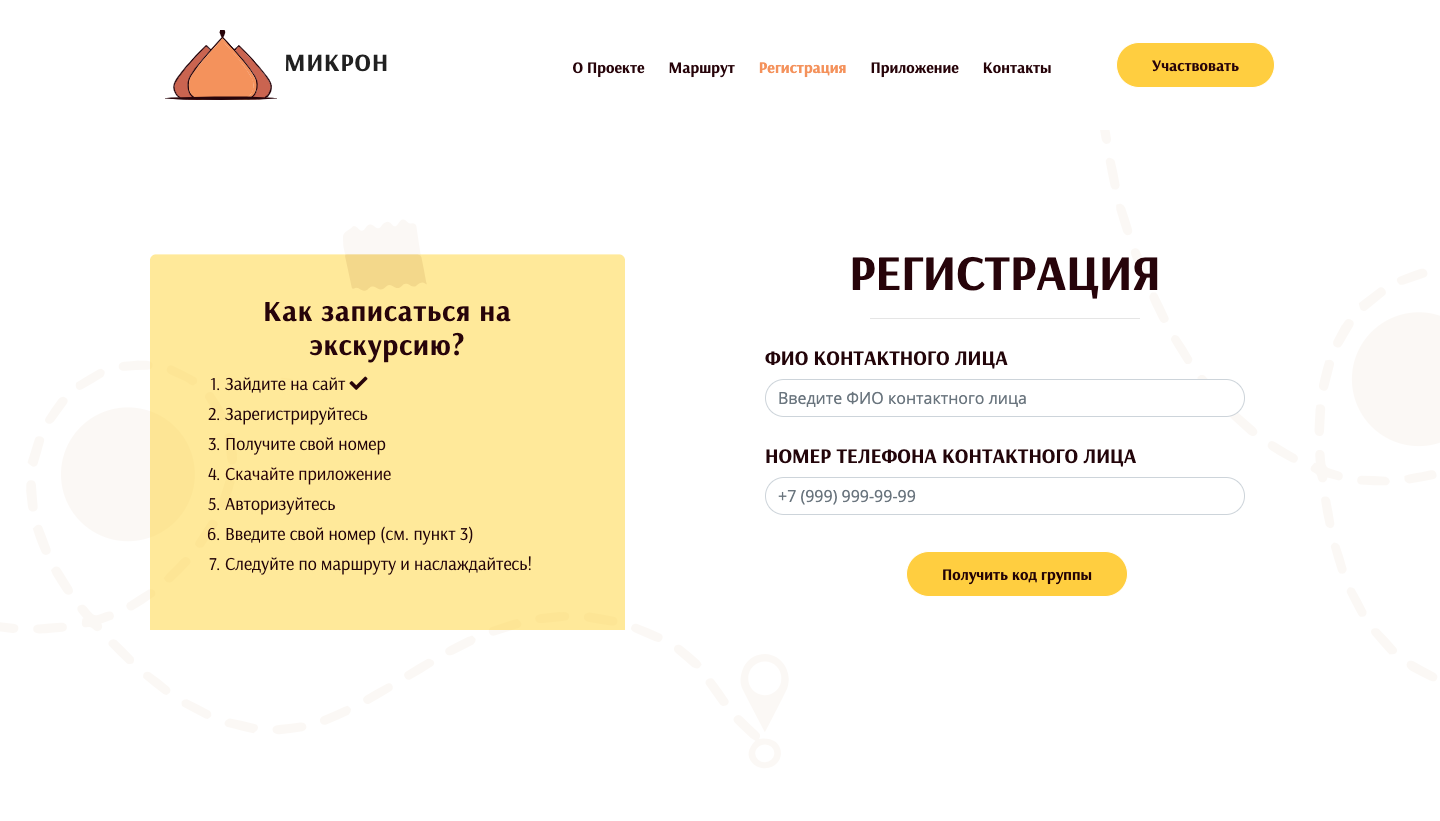
\includegraphics[width=11cm]{4}} \\
    \hline
    \multicolumn{3}{|c|}{\textbf{Модель}} \\
    \hline
    \multicolumn{3}{|c|}{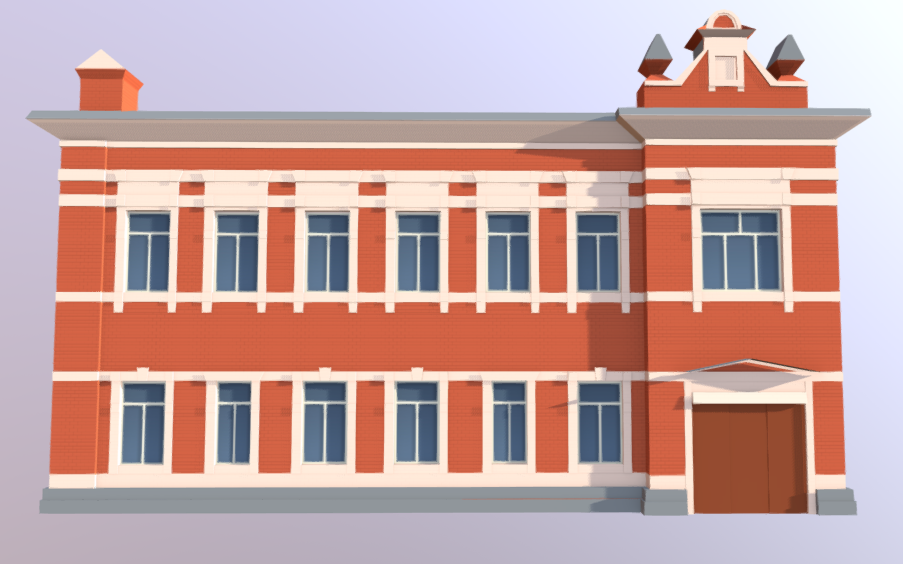
\includegraphics[width=11cm]{src/model_5}} \\
    \hline
    \textbf{Критерий} & \textbf{Балл/ Max.балл} & \textbf{Комментарии} \\
    \hline
    Количество полигонов < 3k. & 0.9/0.9 & Количество полигонов - 1 911, соответствует допустимому диапазону. \\
    \hline
    Детализация. & 0.7/0.7 & Модель не является примитивом, отдельные части не перегружены лишними деталями, детализация не влияет на критерий количества полигонов. \\
    \hline
    Сходство с реальным объектом. & 0.7/0.7 & Объект можно легко опознать при сравнении с оригиналом - сохранены общие пропорции здания, характерные детали и количественный фактор (окна, двери и т.п.) \\
    \hline
    UV-развертка. & 0.6/0.6 & Развертка присутствует. Вес развертки правильный (окрашена в равномерный синий цвет без ярких зеленых или желтых зон).

    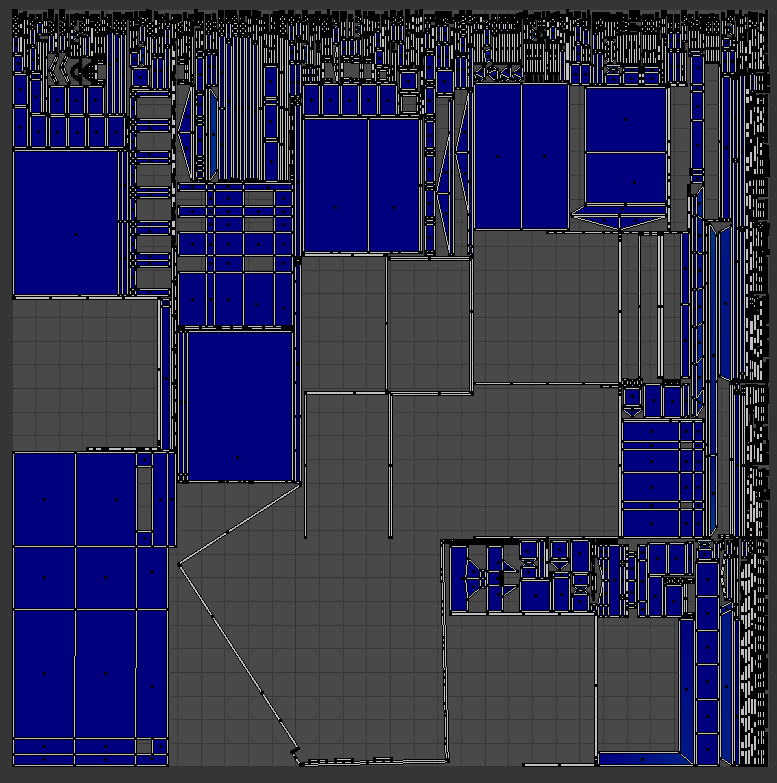
\includegraphics[width=7cm]{src/uv_5} \\
    \hline
    Наличие текстур. & 2.0/2.0 & Текстура присутствует (+ дополнительная текстура для ambient occlusion), все текстурные элементы запечены на одну текстуру.

    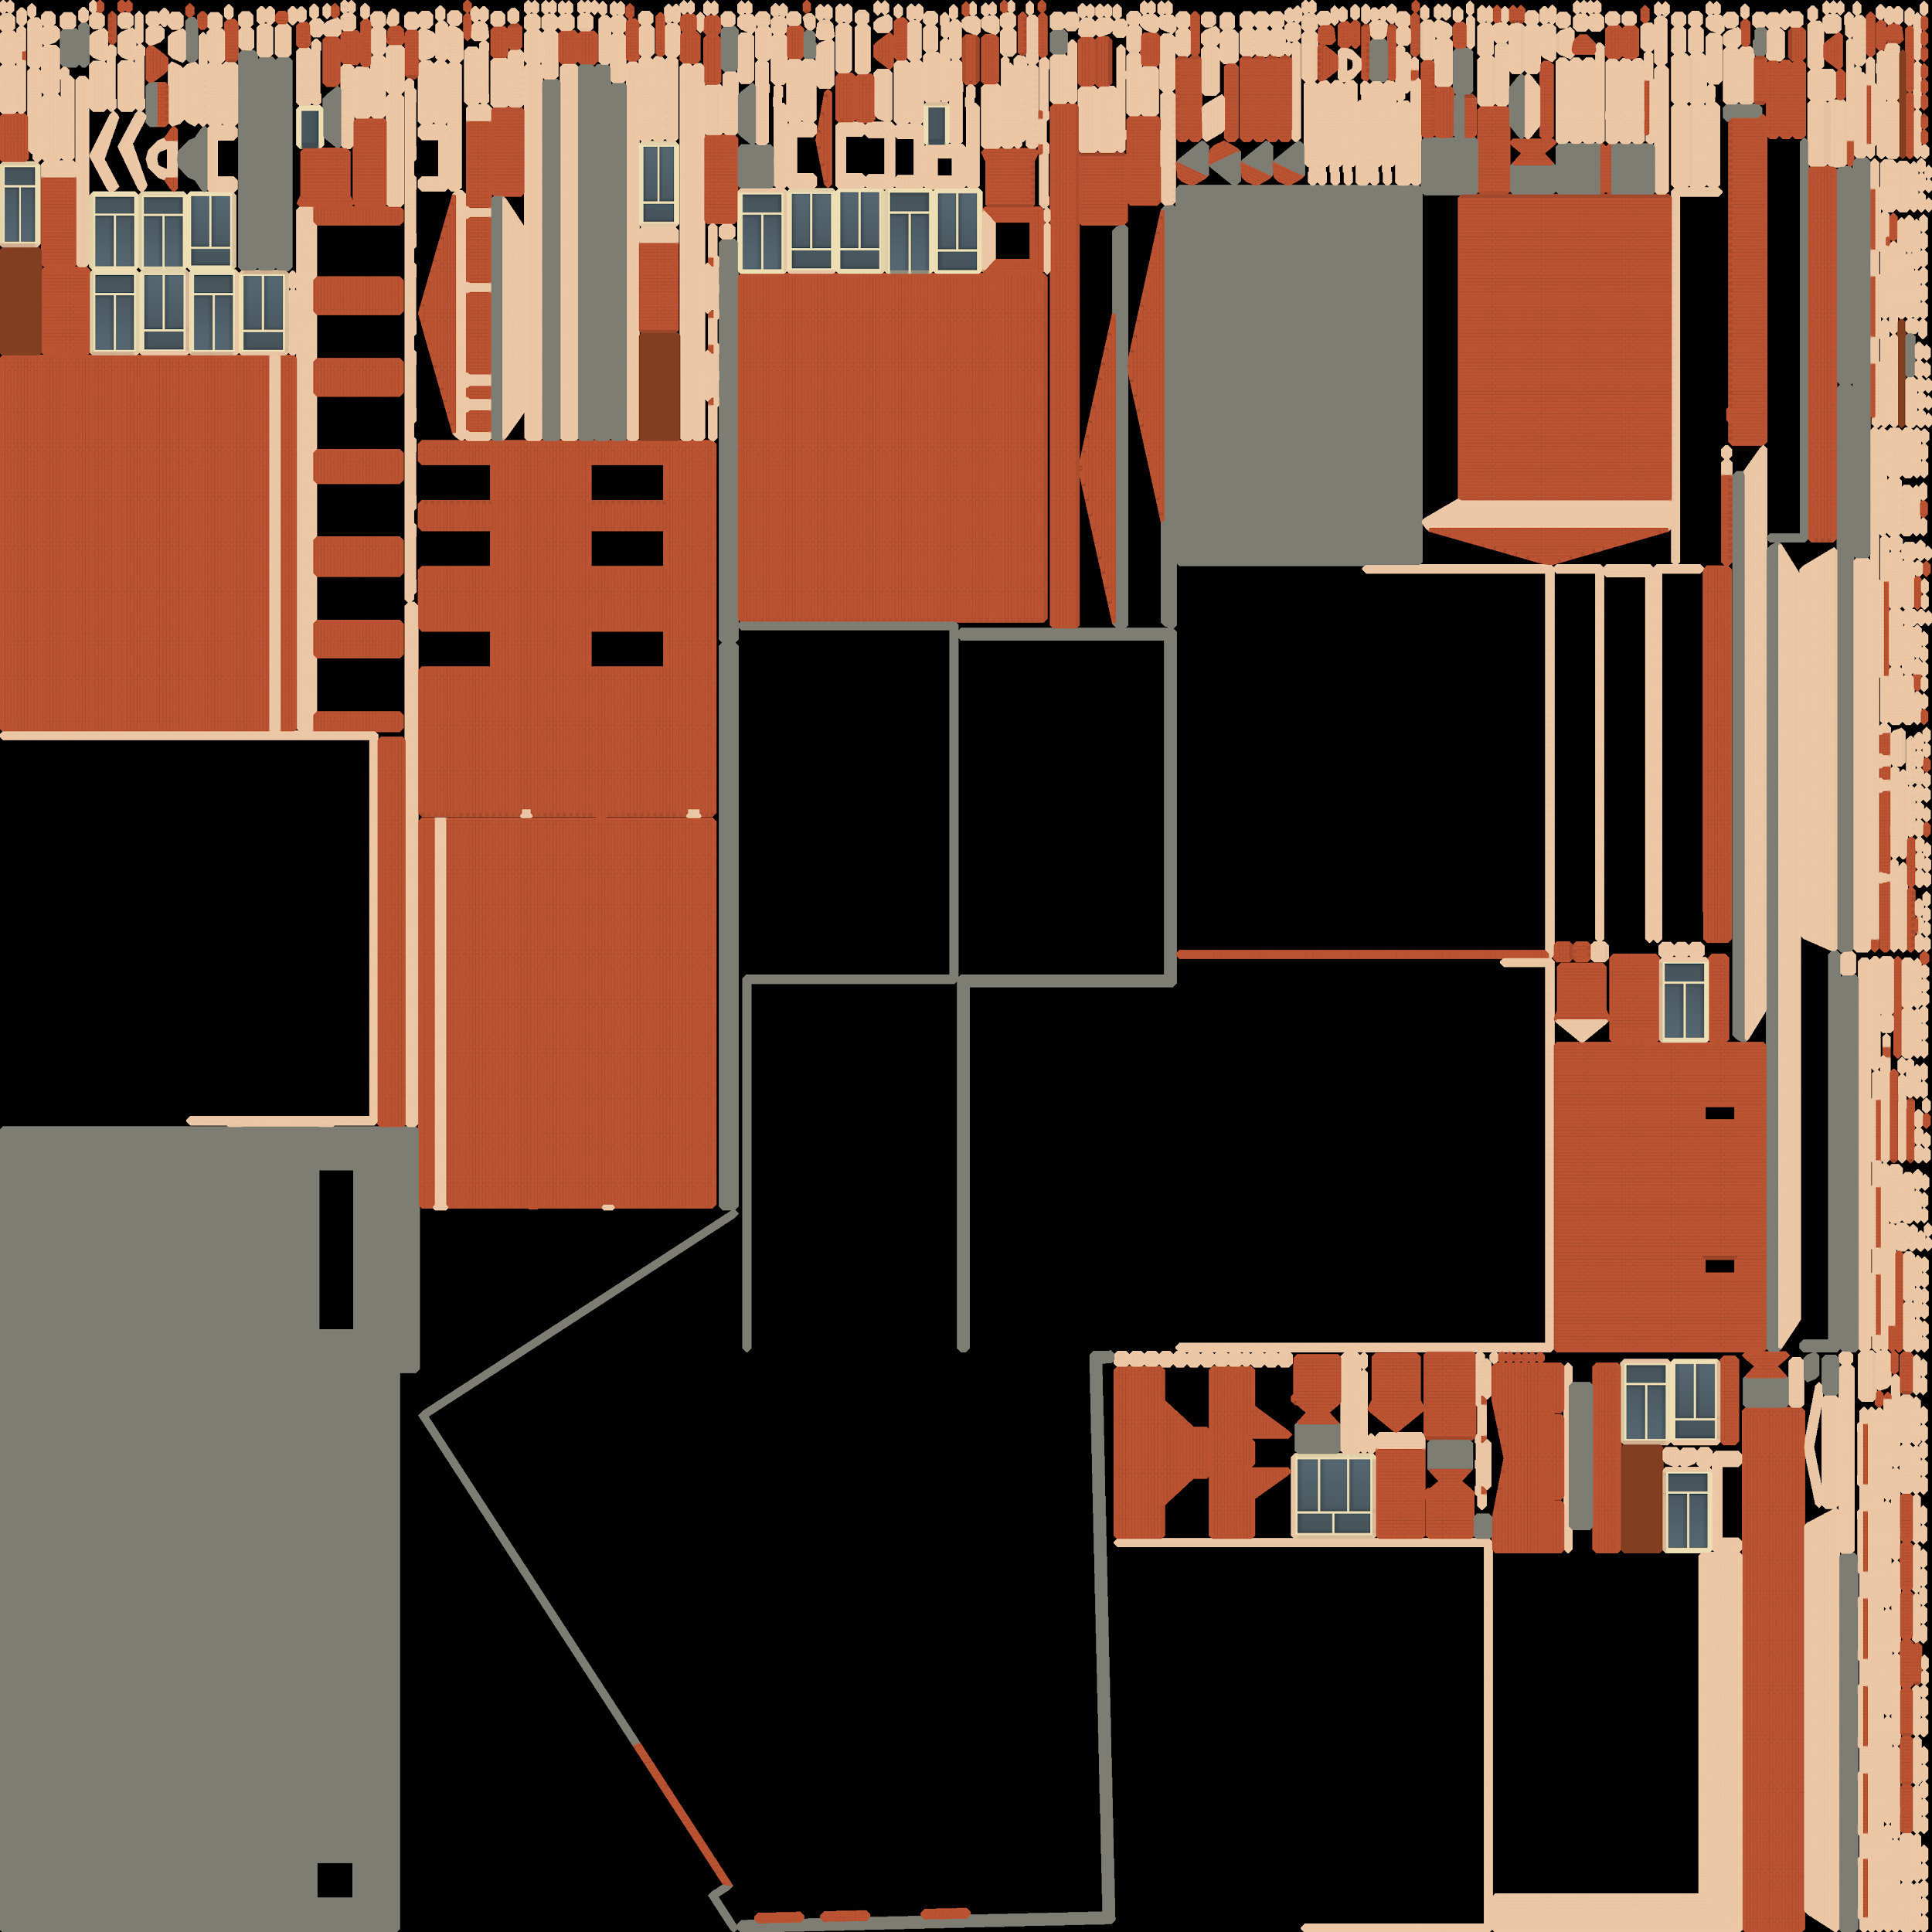
\includegraphics[width=7cm]{src/tec_9}\\
    & & 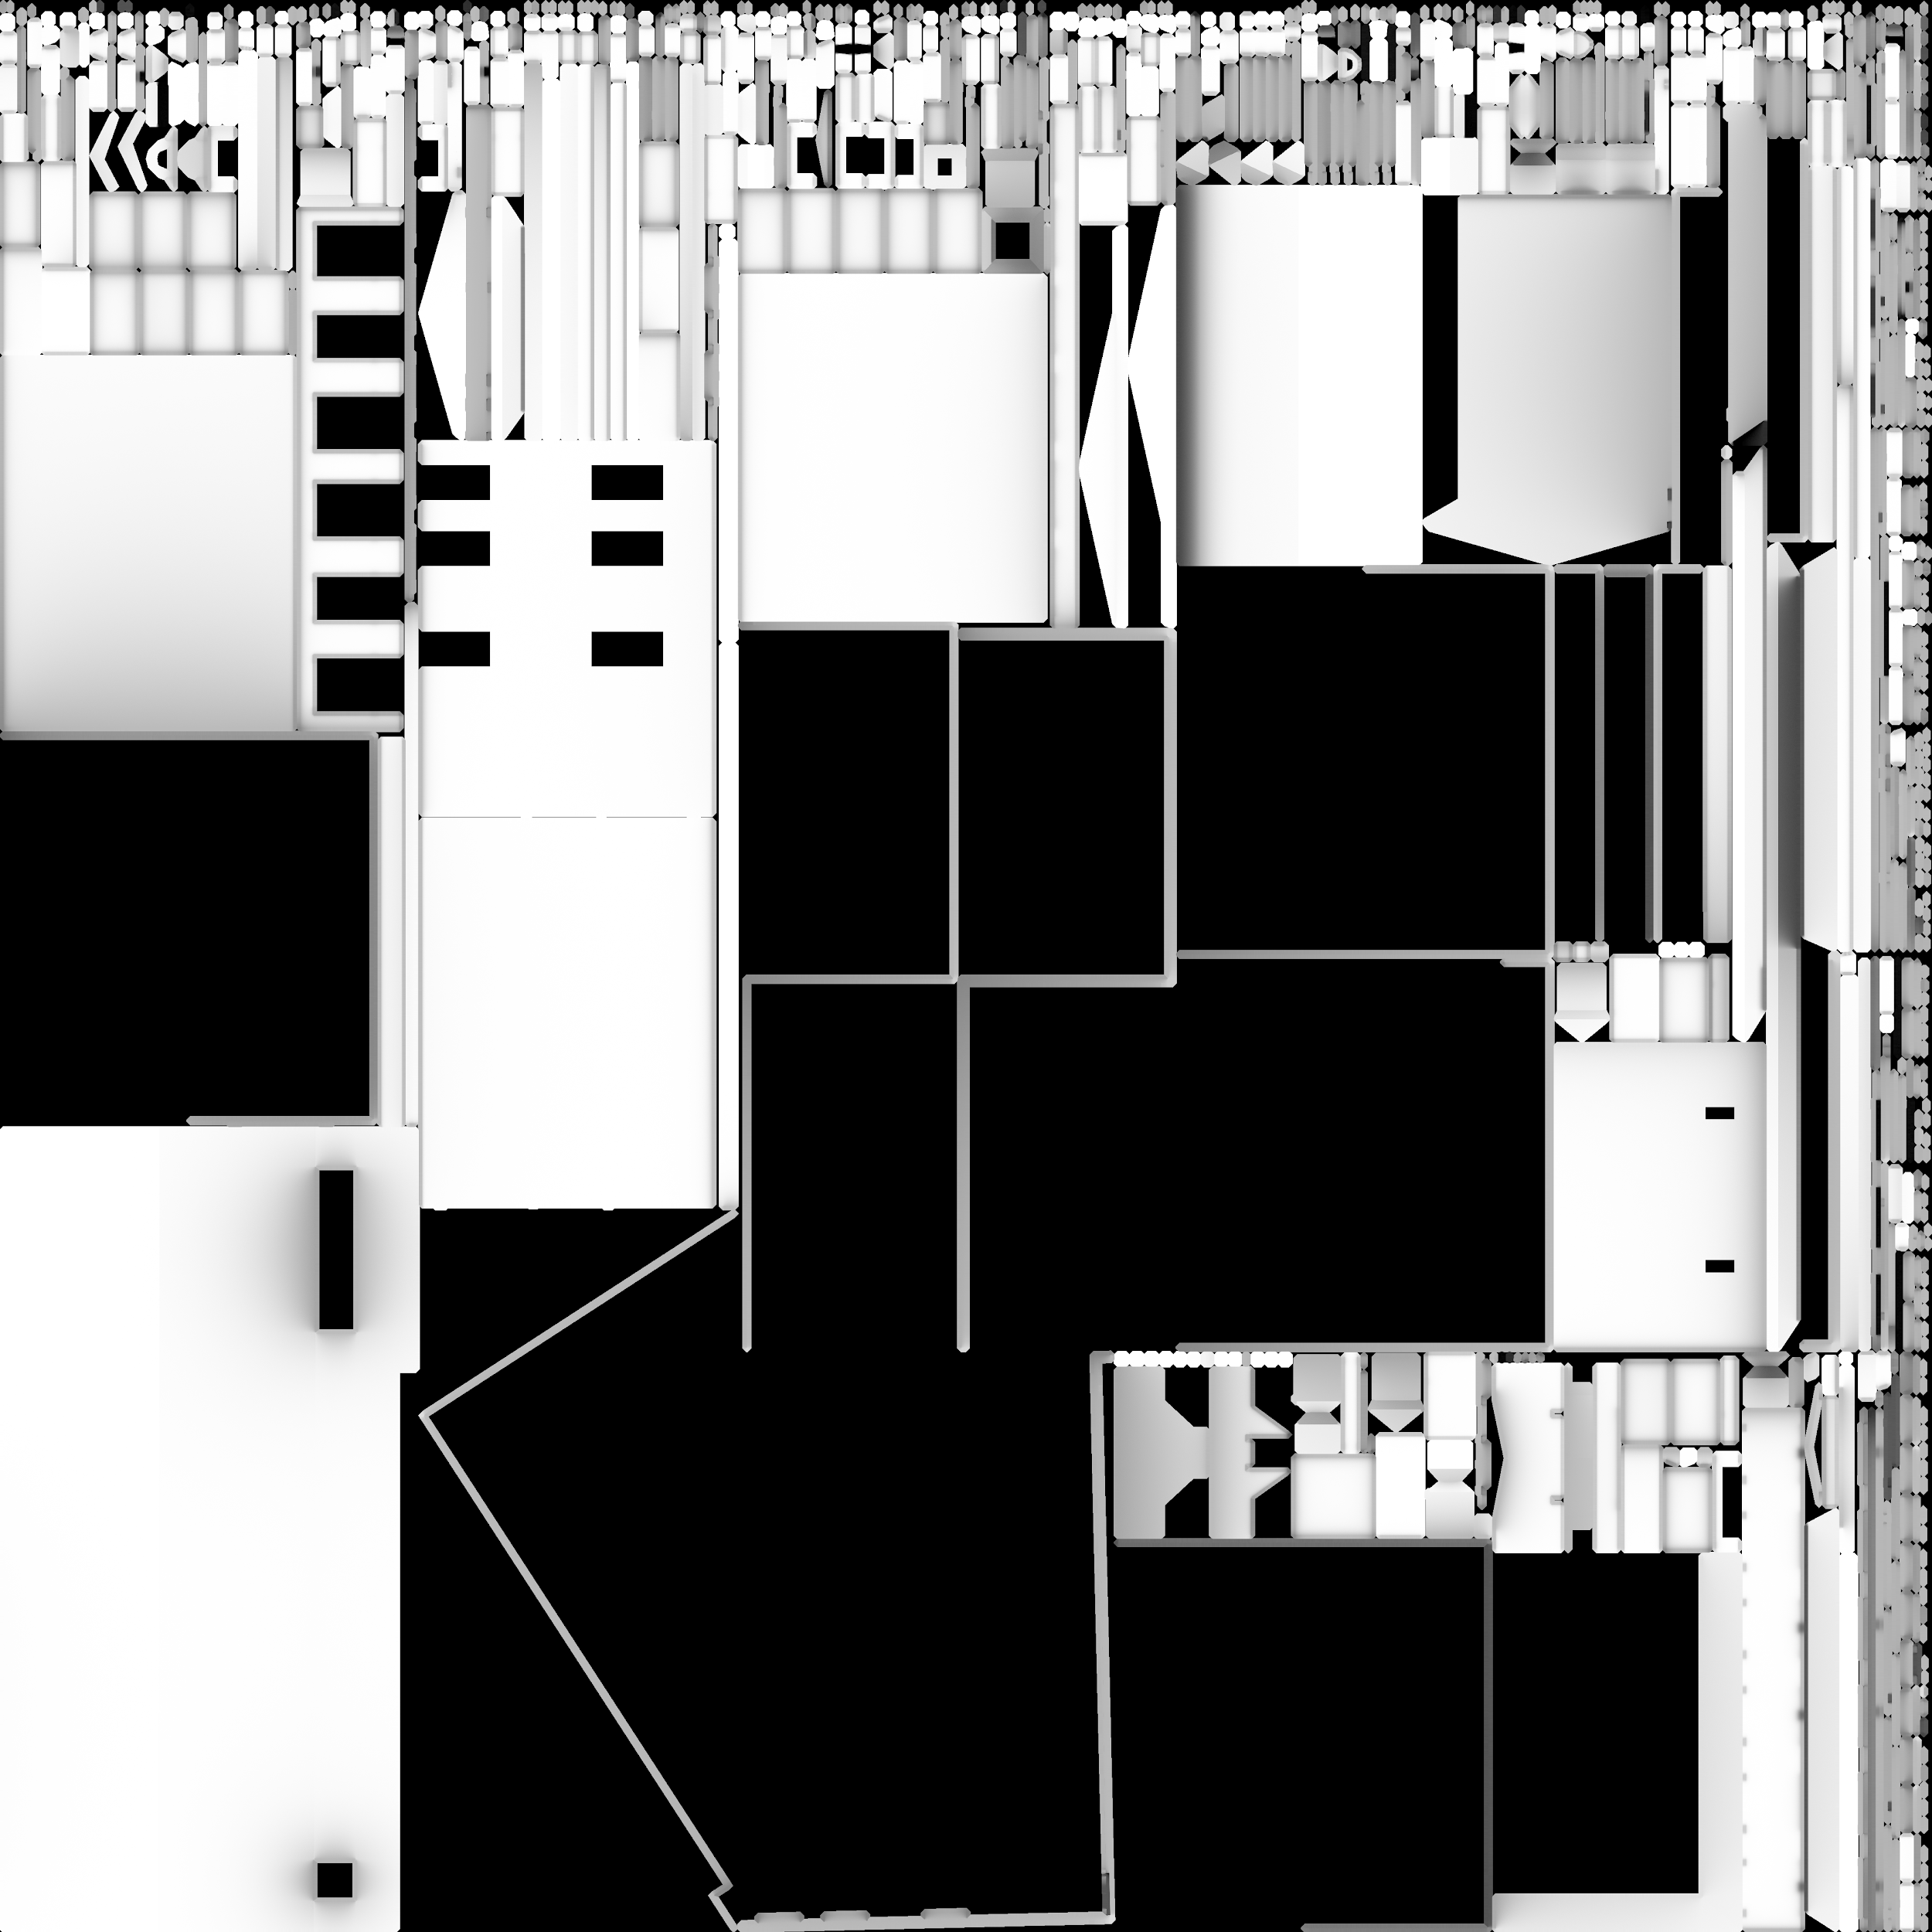
\includegraphics[width=7cm]{src/tec_10} \\
    \hline
    Отсутствие перевернутых нормалей. & 0.45/0.45 & Оси нормалей отображаются верно, направлены из объекта, а не вовнутрь. Нет затемненных участков меша или участков объекта без отображаемых текстур (свидетельство перевернутых нормалей).
 
    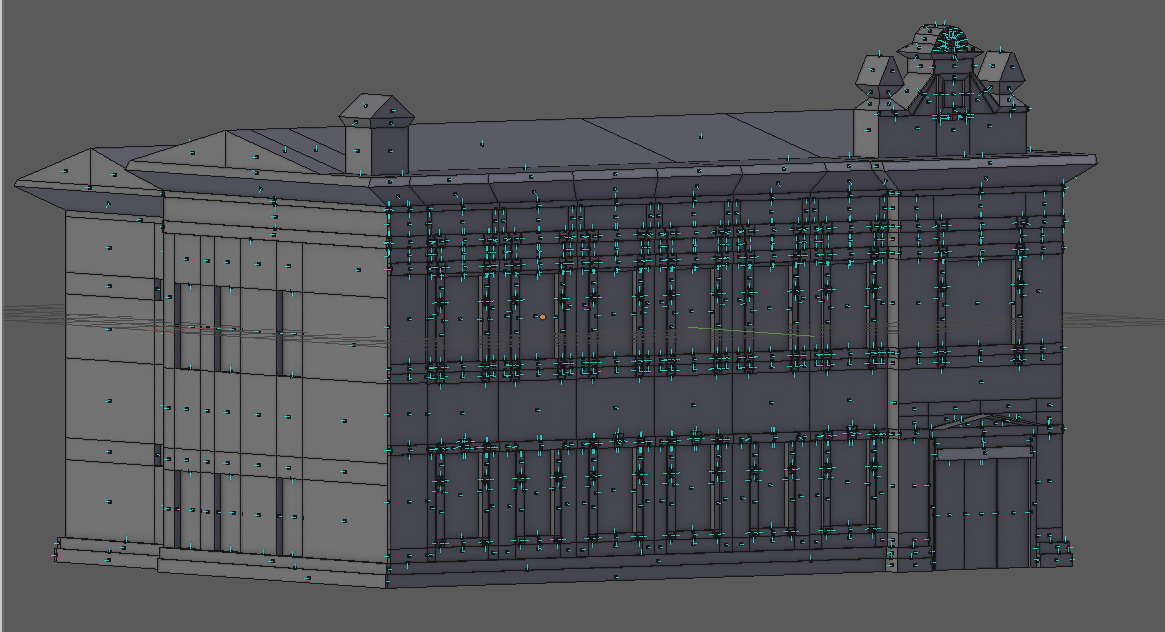
\includegraphics[width=7cm]{src/norm_9}\\
    & & 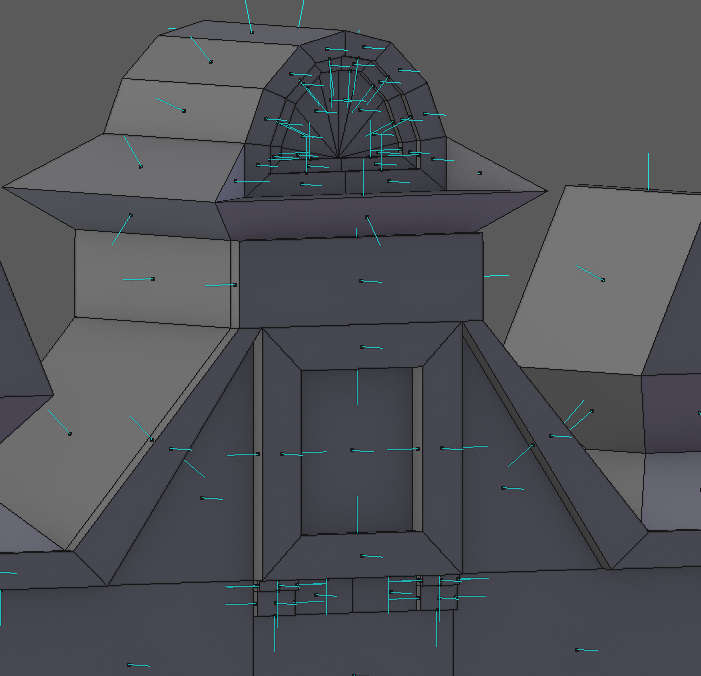
\includegraphics[width=7cm]{src/norm_10}\\
    \hline
    Отсутствие неправильных полигонов. & 0.6/0.6 & Все полигоны имеют форму четырехугольника или треугольника, нет полигонов с большим количеством углов. \\
    \hline
    \multicolumn{3}{|c|}{\textbf{Итого за модель: 5.95}} \\
    \hline
\end{longtable}

\begin{center}
    \textbf{Модель №6}
\end{center}

\begin{longtable}{|p{4cm}|p{2.5cm}|p{7.5cm}|}
    \hline
    \multicolumn{3}{|c|}{\textbf{Оригинальное здание} } \\
    \hline
    \multicolumn{3}{|c|}{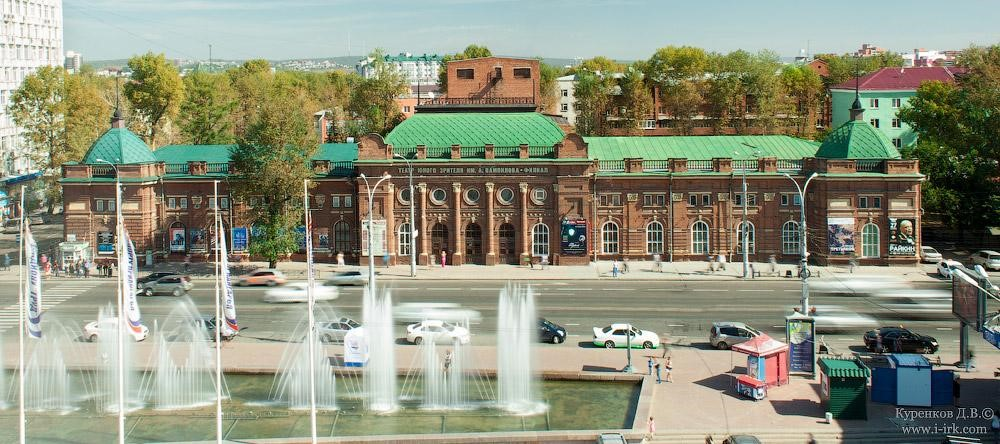
\includegraphics[width=11cm]{src/build_6}} \\
    \hline
    \multicolumn{3}{|c|}{\textbf{Модель}} \\
    \hline
    \multicolumn{3}{|c|}{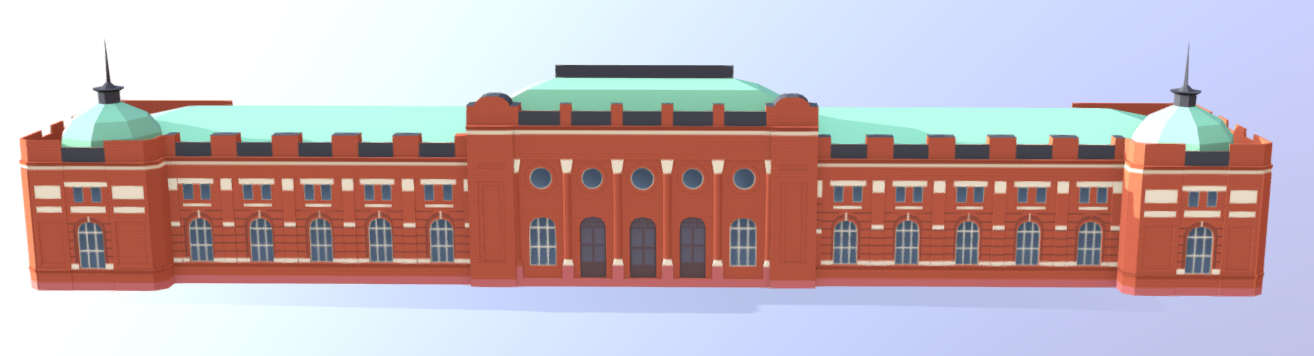
\includegraphics[width=11cm]{src/model_6}} \\
    \hline
    \textbf{Критерий} & \textbf{Балл/ Max.балл} & \textbf{Комментарии} \\
    \hline
    Количество полигонов < 3k. & 0.9/0.9 & Количество полигонов - 2 847, соответствует допустимому диапазону. \\
    \hline
    Детализация. & 0.7/0.7 & Модель не является примитивом, отдельные части не перегружены лишними деталями, детализация не влияет на критерий количества полигонов. \\
    \hline
    Сходство с реальным объектом. & 0.7/0.7 & Объект можно легко опознать при сравнении с оригиналом - сохранены общие пропорции здания, характерные детали и количественный фактор (окна, двери и т.п.) \\
    \hline
    UV-развертка. & 0.6/0.6 & Развертка присутствует. Вес развертки правильный (окрашена в равномерный синий цвет без ярких зеленых или желтых зон).

    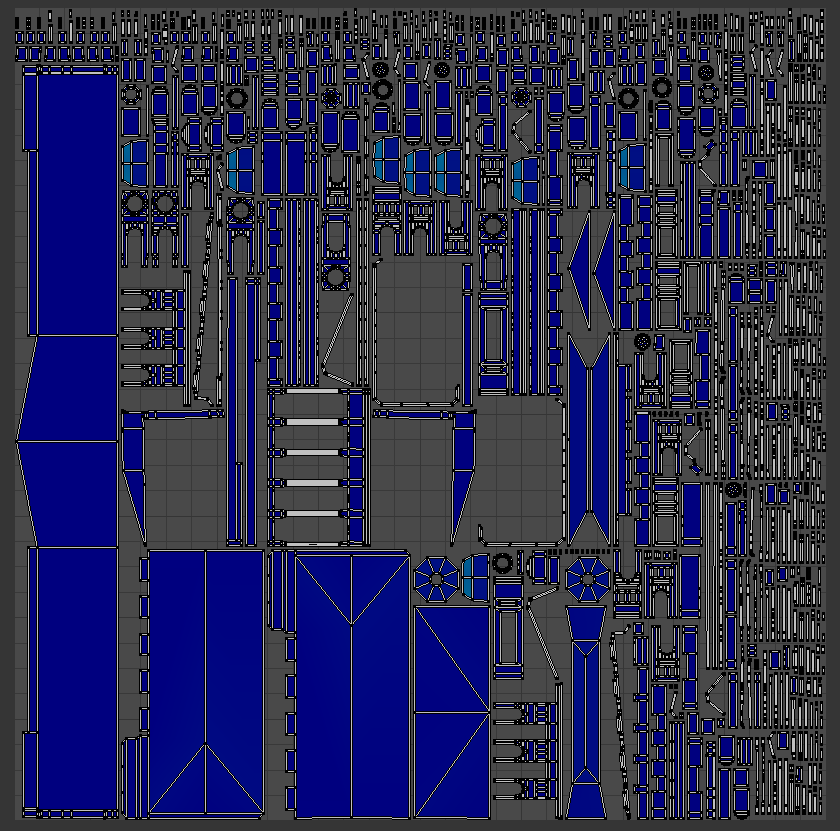
\includegraphics[width=7cm]{src/uv_6} \\
    \hline   
    Наличие текстур. & 2.0/2.0 & Текстура присутствует (+ дополнительная текстура для ambient occlusion), все текстурные элементы запечены на одну текстуру.

    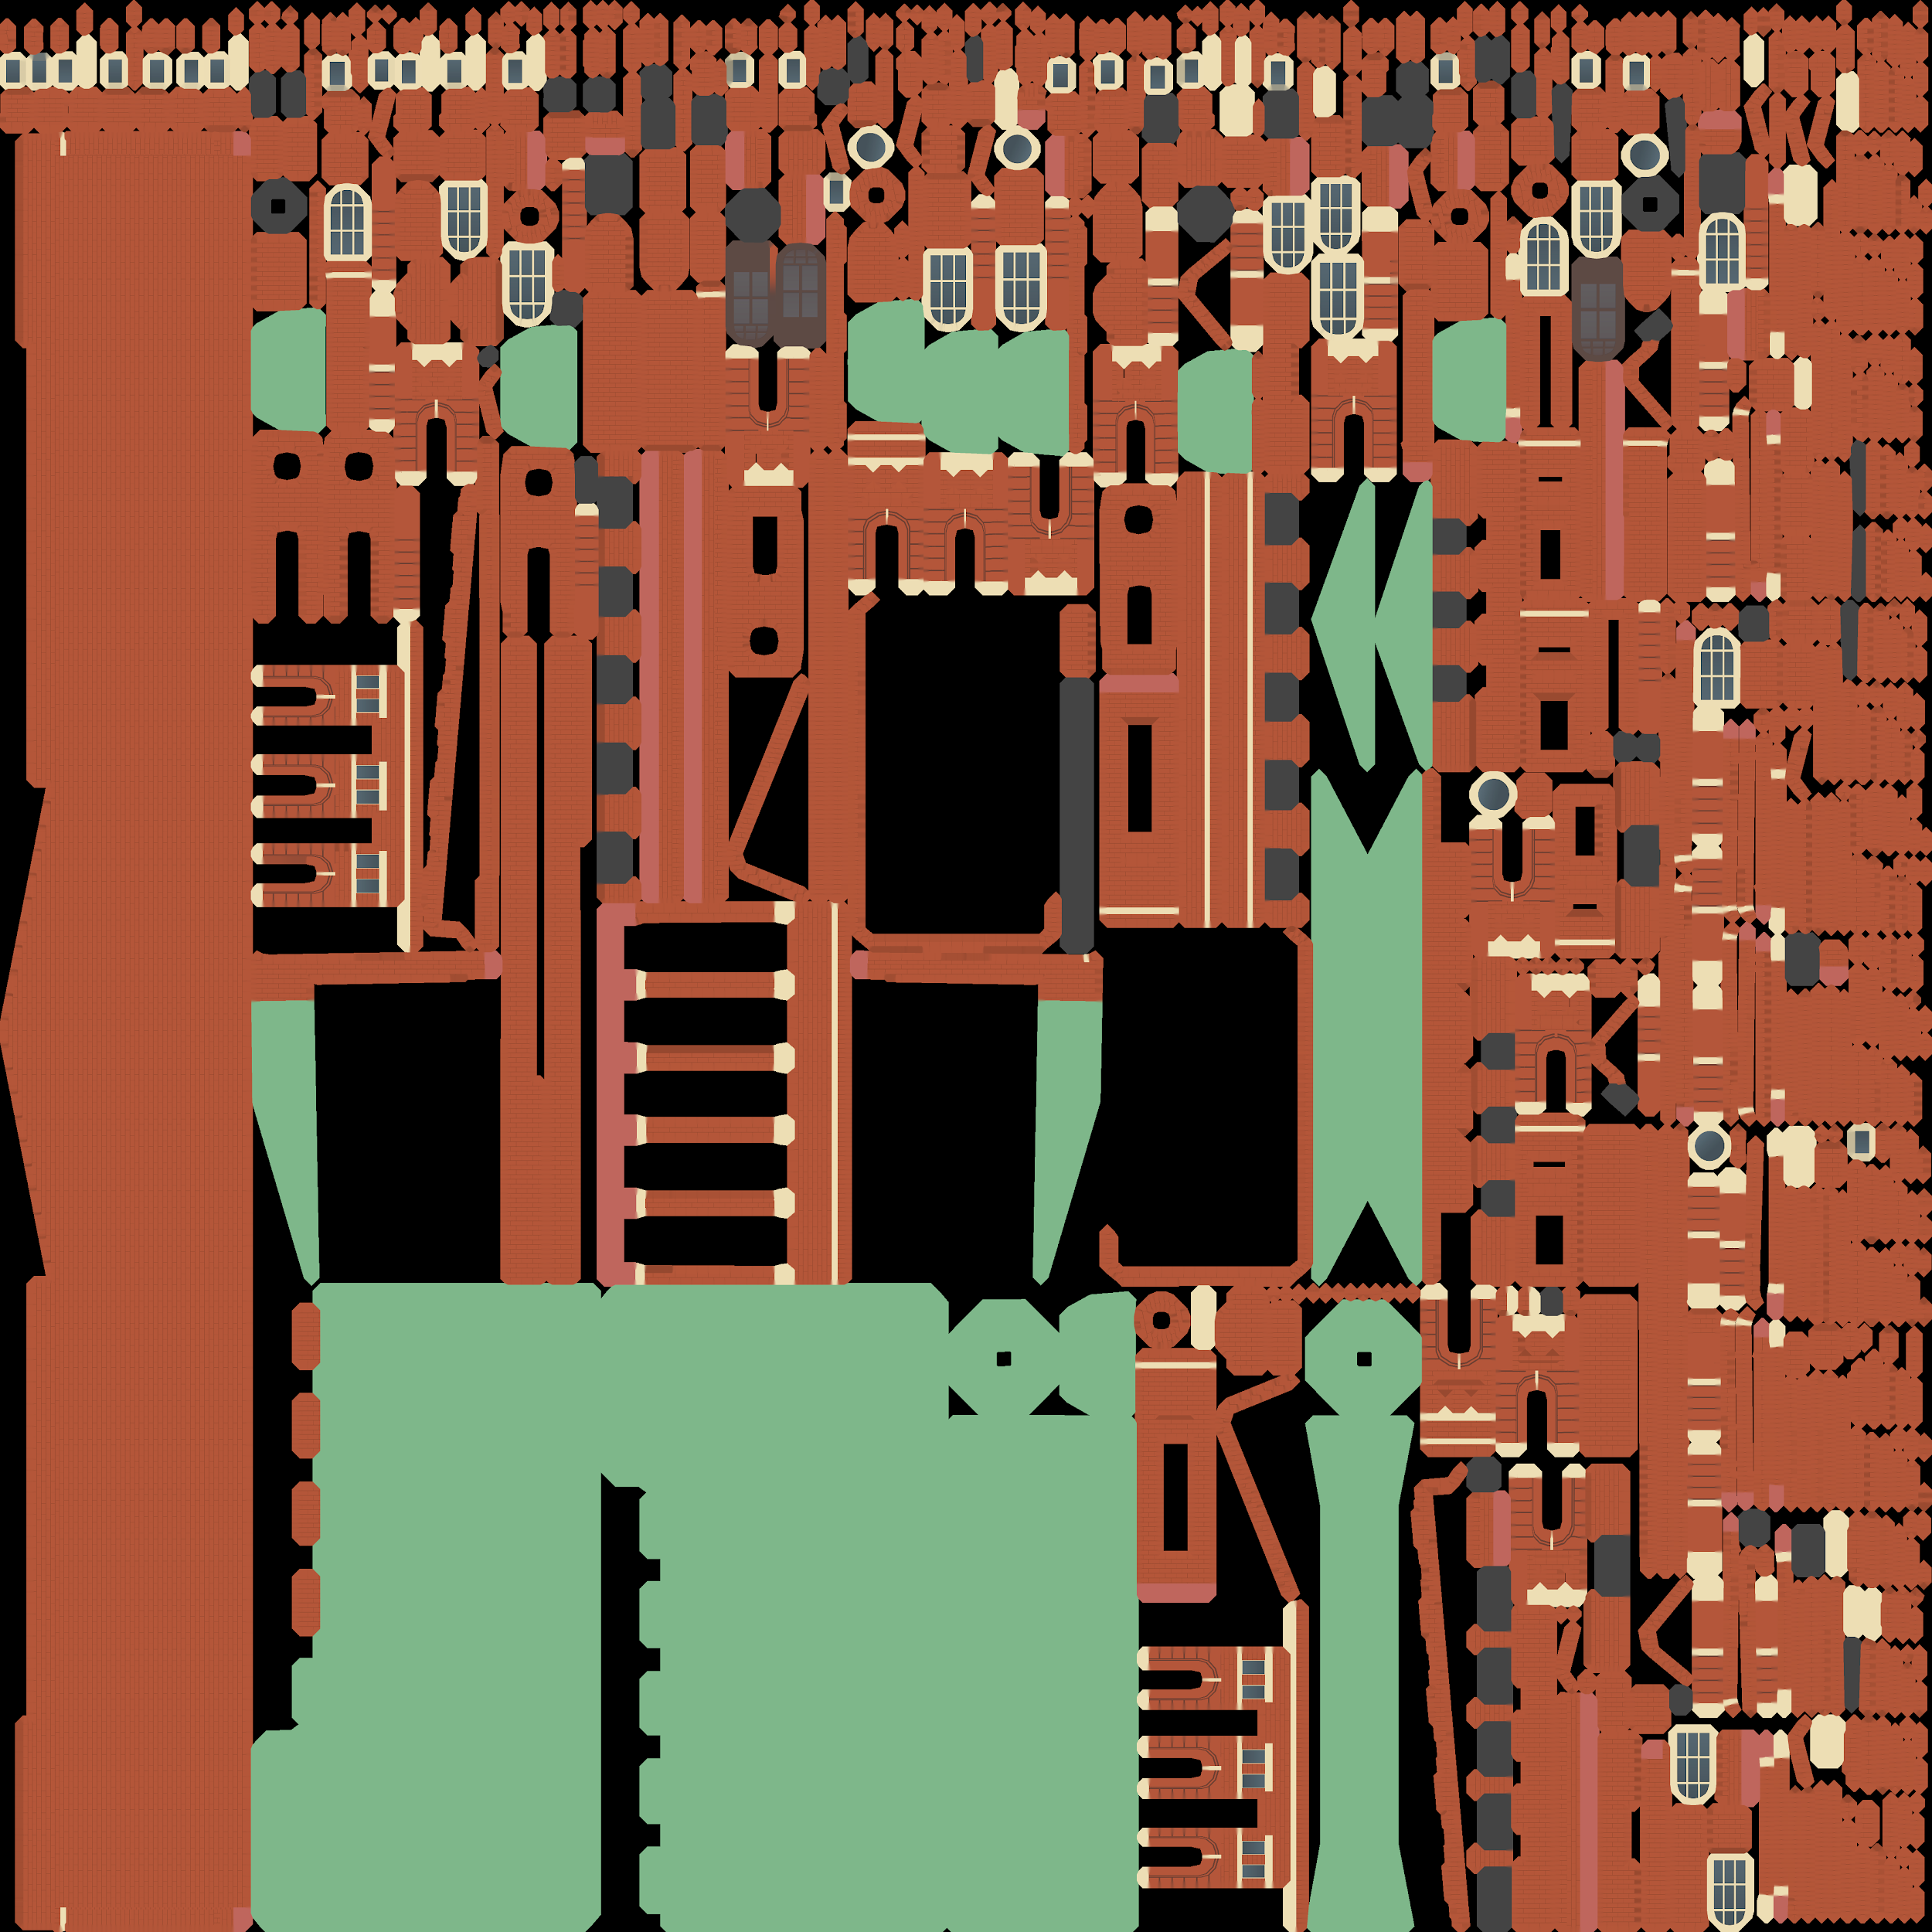
\includegraphics[width=7cm]{src/tec_11}\\
    & & 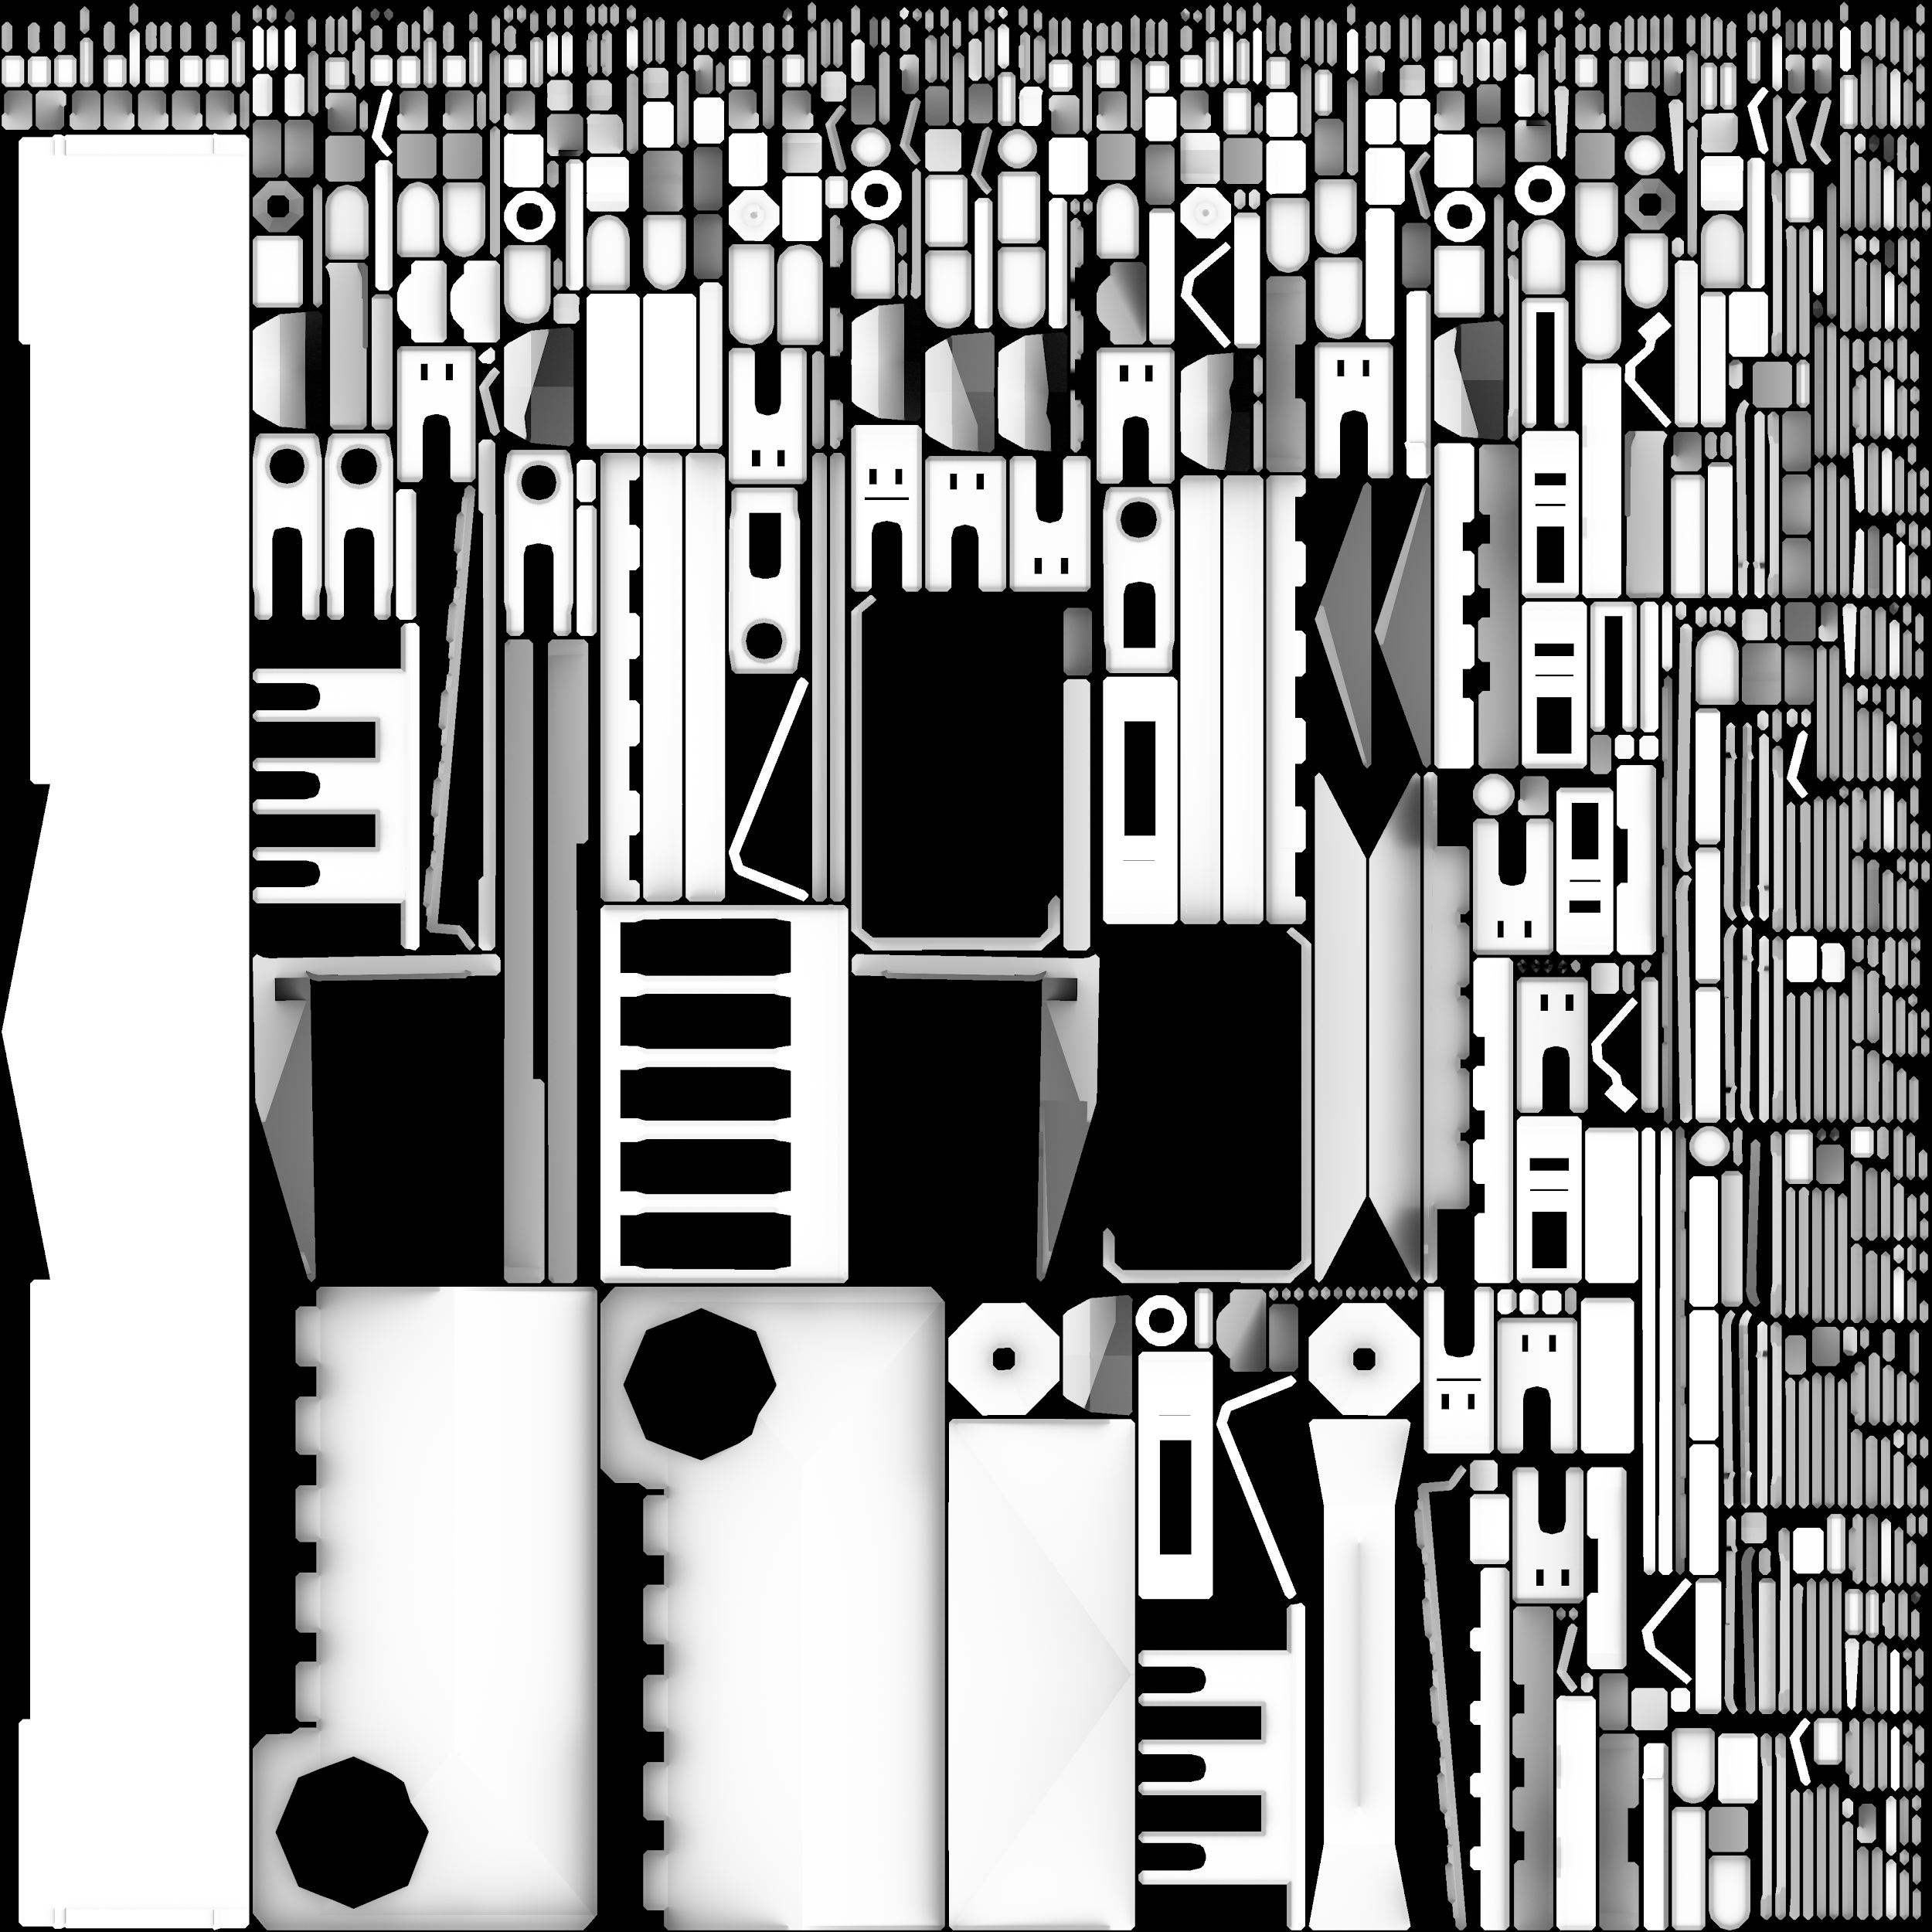
\includegraphics[width=7cm]{src/tec_12} \\
    \hline    
    Отсутствие перевернутых нормалей. & 0.45/0.45 & Оси нормалей отображаются верно, направлены из объекта, а не вовнутрь. Нет затемненных участков меша или участков объекта без отображаемых текстур (свидетельство перевернутых нормалей).

    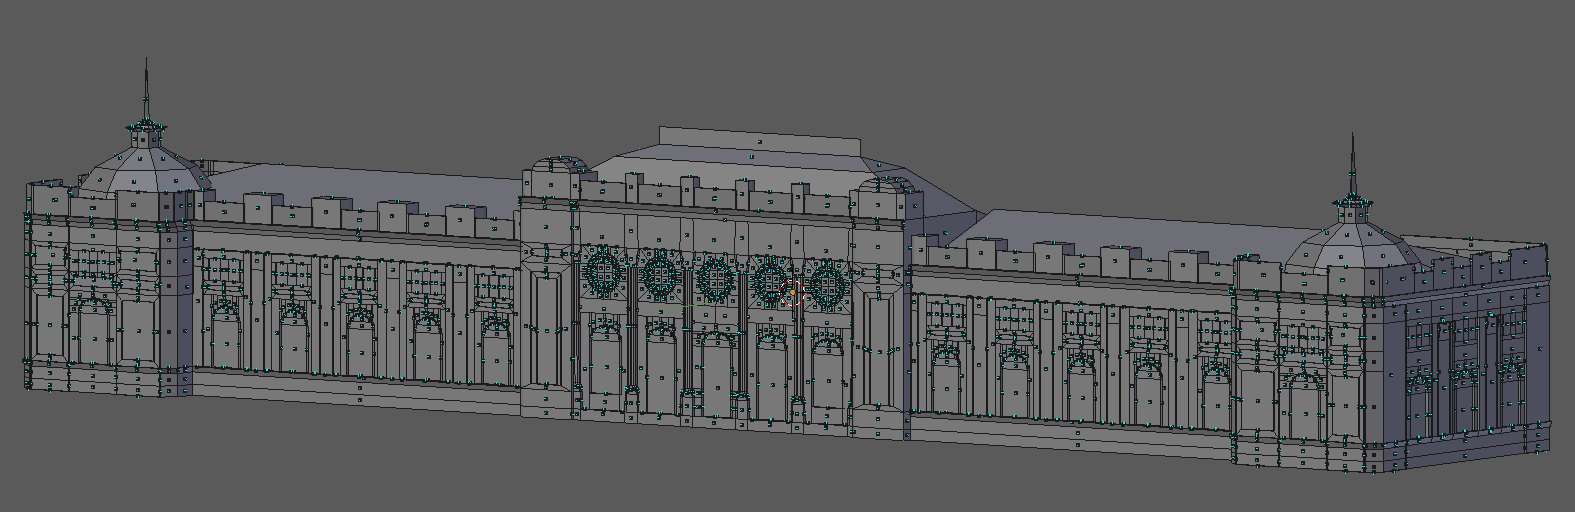
\includegraphics[width=7cm]{src/norm_11}\\
    & & 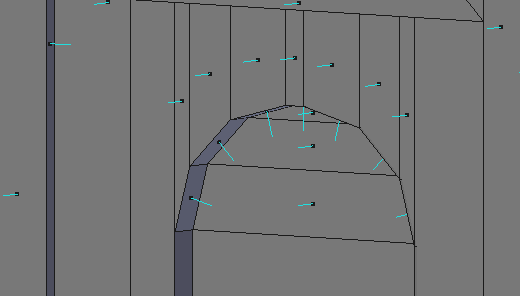
\includegraphics[width=7cm]{src/norm_12} \\
    \hline     
    Отсутствие неправильных полигонов. & 0.6/0.6 & Все полигоны имеют форму четырехугольника или треугольника, нет полигонов с большим количеством углов. \\
    \hline
    \multicolumn{3}{|c|}{\textbf{Итого за модель: 5.95}} \\
    \hline
\end{longtable}

\begin{center}
    \textbf{Модель №7}
\end{center}

\begin{longtable}{|p{4cm}|p{2.5cm}|p{7.5cm}|}
    \hline
    \multicolumn{3}{|c|}{\textbf{Оригинальное здание} } \\
    \hline
    \multicolumn{3}{|c|}{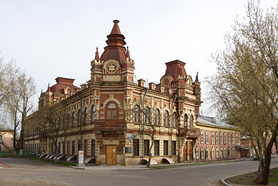
\includegraphics[width=11cm]{6}} \\
    \hline
    \multicolumn{3}{|c|}{\textbf{Модель}} \\
    \hline
    \multicolumn{3}{|c|}{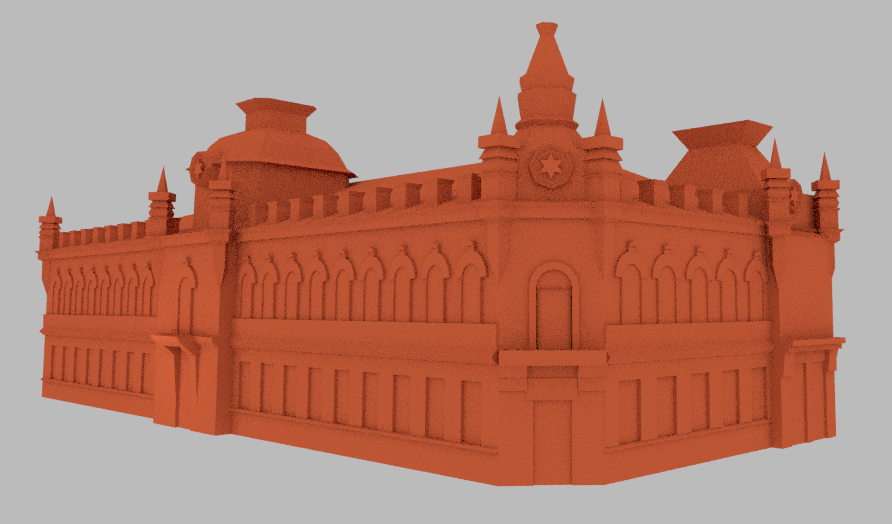
\includegraphics[width=11cm]{src/model_7}} \\
    \hline
    \textbf{Критерий} & \textbf{Балл/ Max.балл} & \textbf{Комментарии} \\
    \hline
    Количество полигонов < 3k. & 0.9/0.9 & Количество полигонов - 2 980, соответствует допустимому диапазону. \\
    \hline
    Детализация. & 0.7/0.7 & Модель не является примитивом, отдельные части не перегружены лишними деталями, детализация не влияет на критерий количества полигонов. \\
    \hline
    Сходство с реальным объектом. & 0.35/0.7 & Объект можно легко опознать при сравнении с оригиналом - сохранены общие пропорции здания, характерные детали и количественный фактор (окна, двери и т.п.). Отсутствует характерная для оригинала окраска здания, объект является одноцветным. \\
    \hline
    UV-развертка. & 0.5/0.6 & Развертка присутствует. Вес развертки преимущественно синего цвета, однако есть области со светло-голубым оттенком, что свидетельствует о небольших искажениях текстур. 

    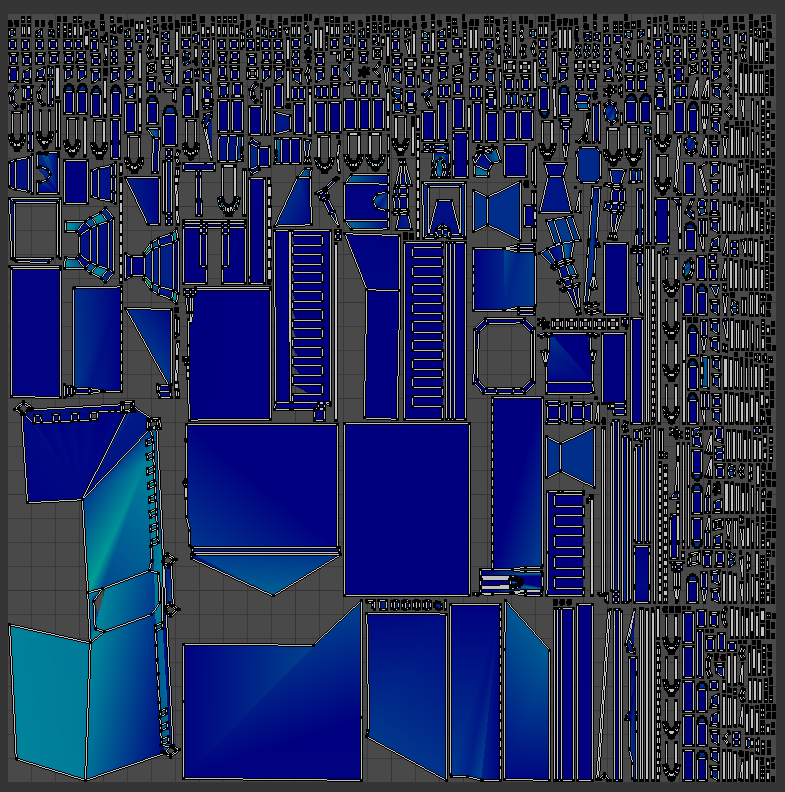
\includegraphics[width=7cm]{src/uv_7}\\
    & & 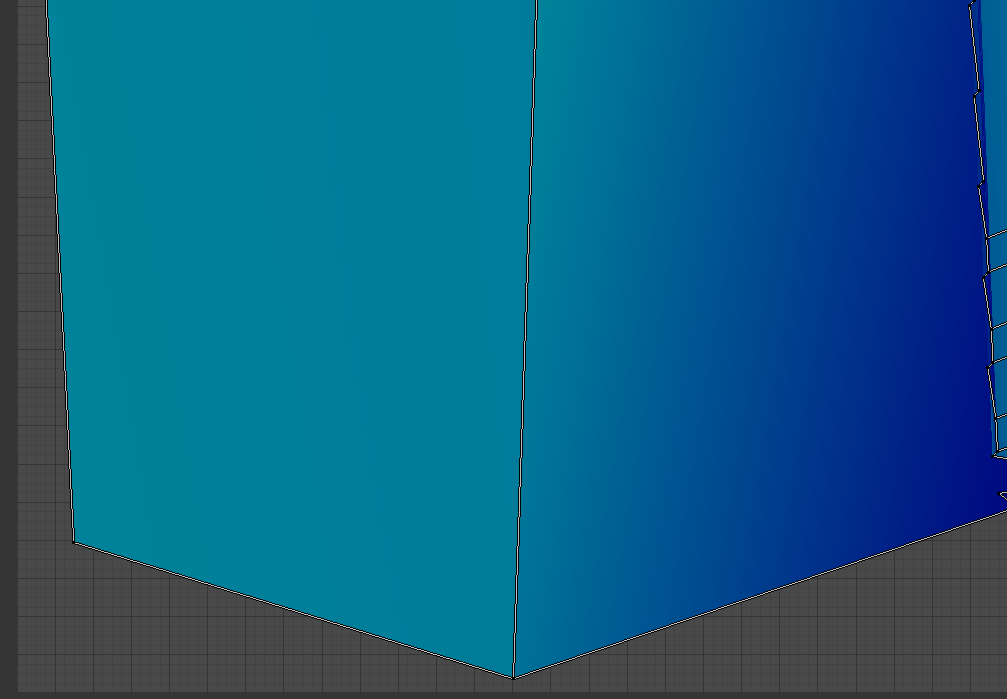
\includegraphics[width=7cm]{src/uv_8}\\
    \hline
    Наличие текстур. & 2.0/2.0 & Текстура присутствует (+ дополнительная текстура для ambient occlusion), все текстурные элементы запечены на одну текстуру.

    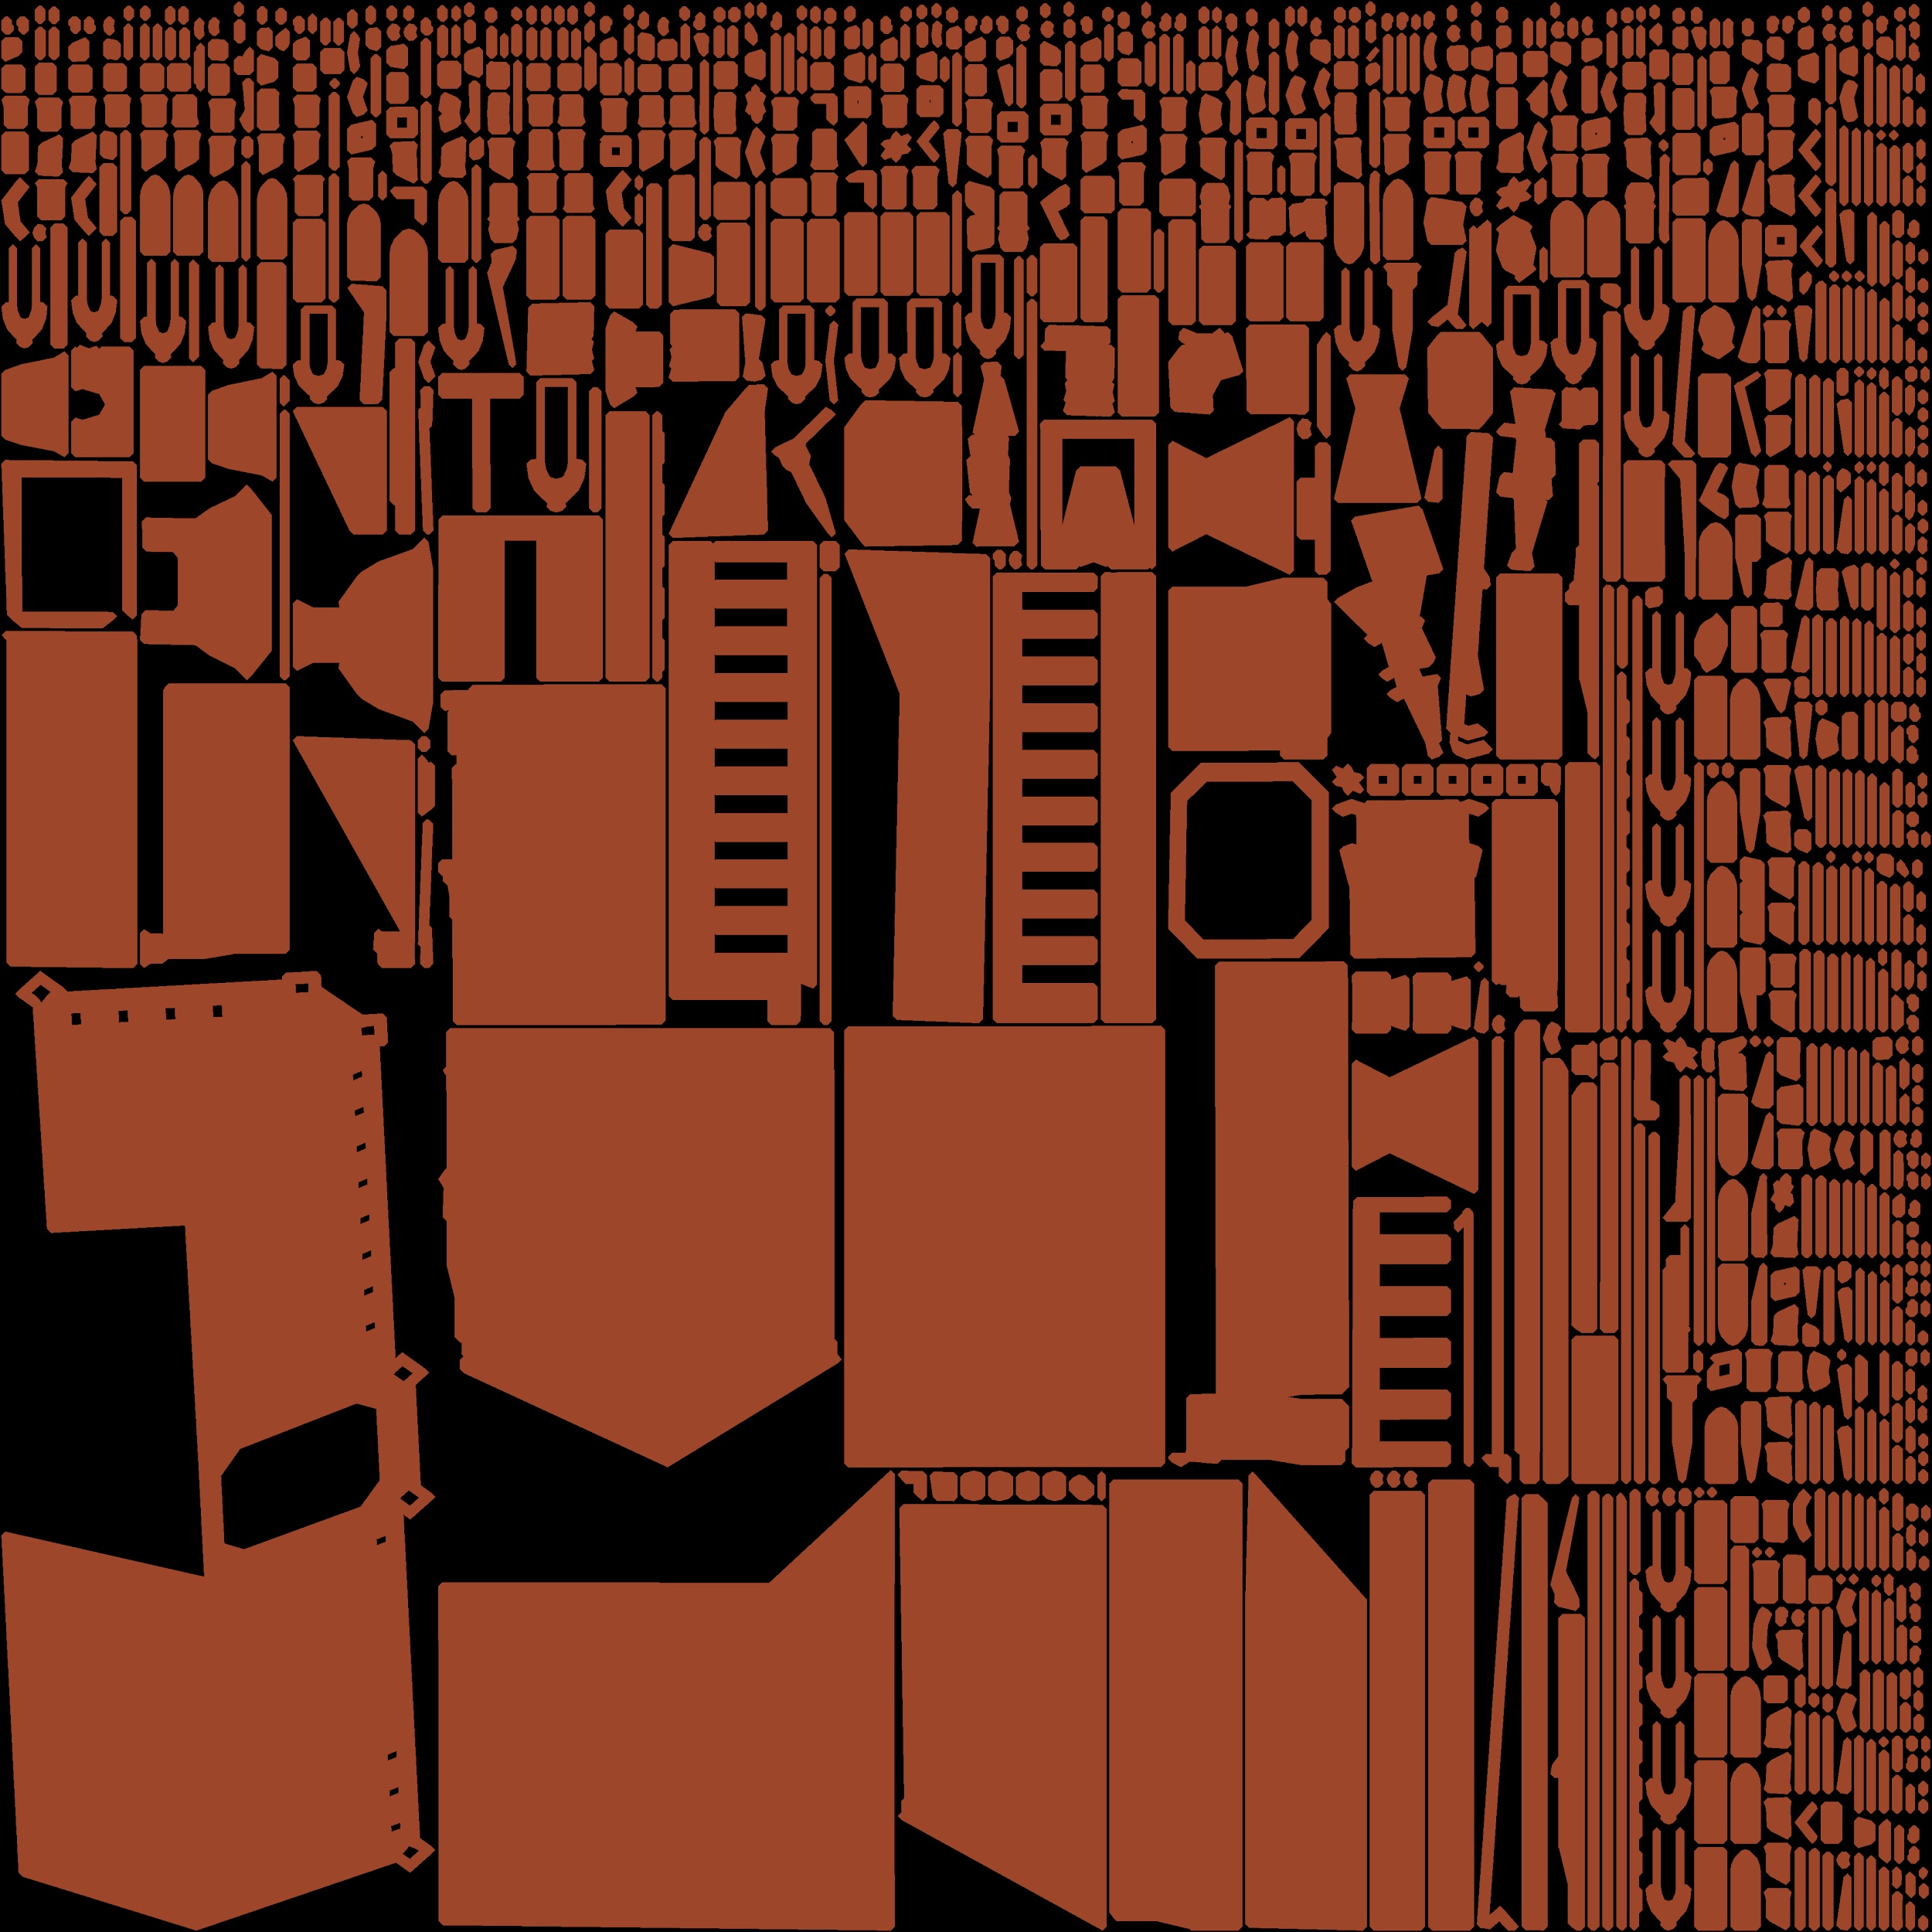
\includegraphics[width=7cm]{src/tec_13}\\
    & & \includegraphics[width=7cm]{src/tec_14}\\
    \hline
    Отсутствие перевернутых нормалей. & 0.45/0.45 & Оси нормалей отображаются верно, направлены из объекта, а не вовнутрь. Нет затемненных участков меша или участков объекта без отображаемых текстур (свидетельство перевернутых нормалей). 
    
    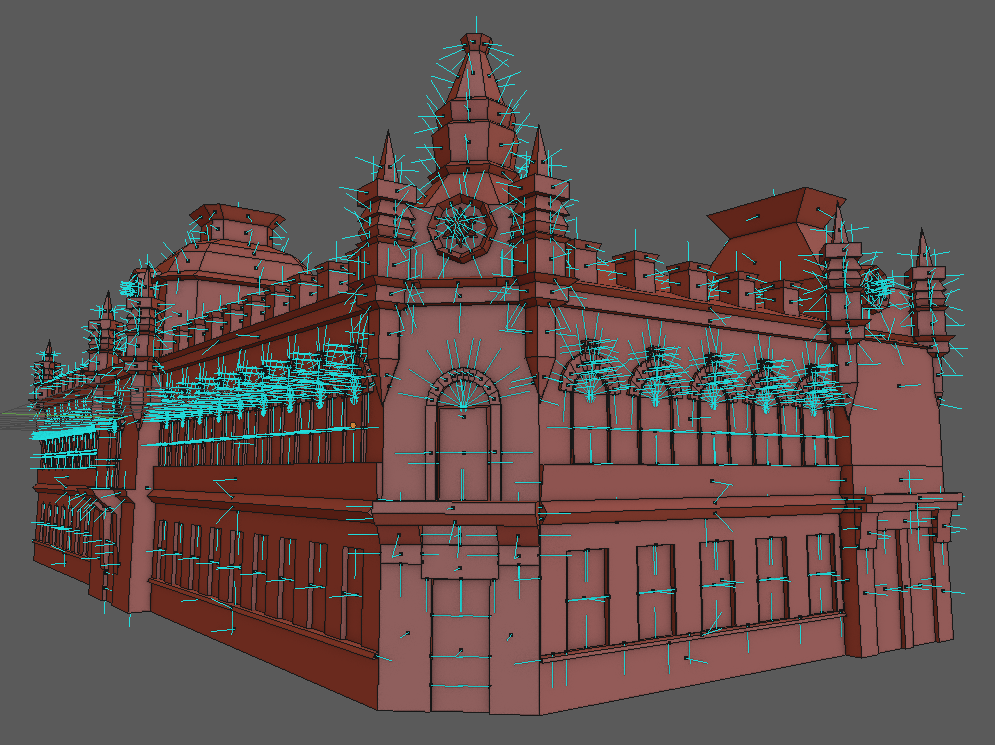
\includegraphics[width=7cm]{src/norm_13}\\
    & & 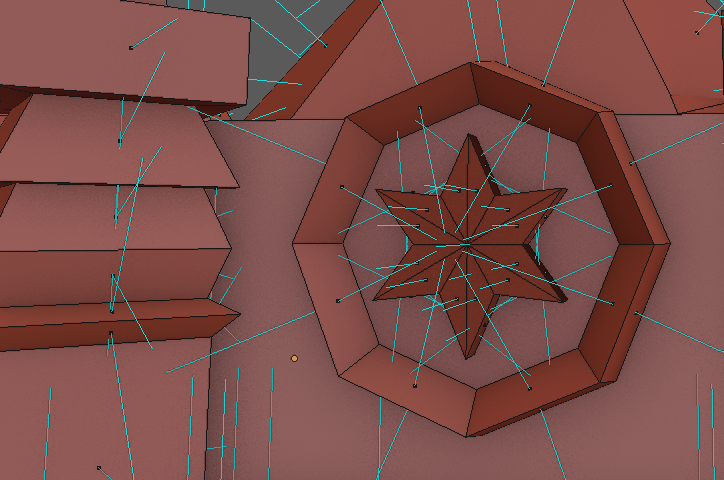
\includegraphics[width=7cm]{src/norm_14}\\
    \hline 
    Отсутствие неправильных полигонов. & 0.0/0.6 & Наличие нескольких полигонов с количеством углов более 4 и/или неправильной формы.

    \includegraphics[width=7cm]{src/poly_7}\\
    \hline
    \multicolumn{3}{|c|}{\textbf{Итого за модель: 4.90}}\\
    \hline
\end{longtable}

\begin{center}
    \textbf{Модель №8}
\end{center}

\begin{longtable}{|p{4cm}|p{2.5cm}|p{7.5cm}|}
    \hline
    \multicolumn{3}{|c|}{\textbf{Оригинальное здание} } \\
    \hline
    \multicolumn{3}{|c|}{\includegraphics[width=11cm]{10}} \\
    \hline
    \multicolumn{3}{|c|}{\textbf{Модель}} \\
    \hline
    \multicolumn{3}{|c|}{\includegraphics[width=11cm]{src/model_8}} \\
    \hline
    \textbf{Критерий} & \textbf{Балл/ Max.балл} & \textbf{Комментарии} \\
    \hline
    Количество полигонов < 3k. & 0.9/0.9 & Количество полигонов - 2 688, соответствует допустимому диапазону. \\
    \hline
    Детализация. & 0.7/0.7 & Модель не является примитивом, отдельные части не перегружены лишними деталями, детализация не влияет на критерий количества полигонов. \\
    \hline
    Сходство с реальным объектом. & 0.35/0.7 & Объект можно легко опознать при сравнении с оригиналом - сохранены общие пропорции здания, характерные детали и количественный фактор (окна, двери и т.п.). Отсутствует характерная для оригинала окраска здания, объект является одноцветным. \\
    \hline
    UV-развертка. & 0.5/0.6 & Развертка присутствует. Вес развертки преимущественно синего цвета, однако есть области со светло-синим оттенком, что свидетельствует о небольших искажениях текстур.

    \includegraphics[width=7cm]{src/uv_9}\\
    & & \includegraphics[width=7cm]{src/uv_10}\\
    \hline
    Наличие текстур. & 2.0/2.0 & Текстура присутствует (+ дополнительная текстура для ambient occlusion), все текстурные элементы запечены на одну текстуру.

    \includegraphics[width=7cm]{src/tec_15}\\
    & & \includegraphics[width=7cm]{src/tec_16}\\
  
    \hline
    Отсутствие перевернутых нормалей. & 0.45/0.45 & Оси нормалей отображаются верно, направлены из объекта, а не вовнутрь. Нет затемненных участков меша или участков объекта без отображаемых текстур (свидетельство перевернутых нормалей).

    \includegraphics[width=7cm]{src/norm_15}\\
    & & \includegraphics[width=7cm]{src/norm_16}\\
    \hline
    Отсутствие неправильных полигонов. & 0.6/0.6 & Все полигоны имеют форму четырехугольника или треугольника, нет полигонов с большим количеством углов. \\
    \hline
    \multicolumn{3}{|c|}{\textbf{Итого за модель: 5.50}} \\
    \hline
\end{longtable}

\begin{center}
    \textbf{Модель №9}
\end{center}

\begin{longtable}{|p{4cm}|p{2.5cm}|p{7.5cm}|}
    \hline
    \multicolumn{3}{|c|}{\textbf{Оригинальное здание} } \\
    \hline
    \multicolumn{3}{|c|}{\includegraphics[width=11cm]{10}} \\
    \hline
    \multicolumn{3}{|c|}{\textbf{Модель}} \\
    \hline
    \multicolumn{3}{|c|}{\includegraphics[width=11cm]{src/model_9}} \\
    \hline
    \textbf{Критерий} & \textbf{Балл/ Max.балл} & \textbf{Комментарии} \\
    \hline
    Количество полигонов < 3k. & 0.0/0.9 & Количество полигонов - 3 290, превышает допустимый диапазон. \\
    \hline
    Детализация. & 0.35/0.7 & Модель не является примитивом, отдельные части имеют ничем не обусловленные лишние полигоны. \\
    \hline 
    Сходство с реальным объектом. & 0.35/0.7 & Объект можно легко опознать при сравнении с оригиналом - сохранены общие пропорции здания, характерные детали, однако некоторые детали изменены - отсутствие двери, слитые окна. \\
    \hline
    UV-развертка. & 0.5/0.6 & Развертка присутствует. Вес развертки преимущественно синего цвета, однако есть области со светло-голубым оттенком, что свидетельствует о небольших искажениях текстур.

    \includegraphics[width=7cm]{src/uv_11}\\
    & & \includegraphics[width=7cm]{src/uv_12}\\
    \hline
    Наличие текстур. & 2.0/2.0 & Текстура присутствует (+ дополнительная текстура для ambient occlusion), все текстурные элементы запечены на одну текстуру. 

    \includegraphics[width=7cm]{src/tec_17}\\
    & & \includegraphics[width=7cm]{src/tec_18}\\
    \hline
    Отсутствие перевернутых нормалей. & 0.45/0.45 & Оси нормалей отображаются верно, направлены из объекта, а не вовнутрь. Нет затемненных участков меша или участков объекта без отображаемых текстур (свидетельство перевернутых нормалей).

    \includegraphics[width=7cm]{src/norm_17}\\
    & & \includegraphics[width=7cm]{src/norm_18}\\
    \hline
    Отсутствие неправильных полигонов. & 0.0/0.6 & Наличие нескольких полигонов с количеством углов более 4 и/или неправильной формы.

    \includegraphics[width=7cm]{src/poly_9} \\
    \hline
    \multicolumn{3}{|c|}{\textbf{Итого за модель: 3.65}}\\
    \hline
\end{longtable}

\begin{center}
    \textbf{Модель №10}
\end{center}

\begin{longtable}{|p{4cm}|p{2.5cm}|p{7.5cm}|}
    \hline
    \multicolumn{3}{|c|}{\textbf{Оригинальное здание} } \\
    \hline
    \multicolumn{3}{|c|}{\includegraphics[width=11cm]{9}} \\
    \hline
    \multicolumn{3}{|c|}{\textbf{Модель}} \\
    \hline
    \multicolumn{3}{|c|}{\includegraphics[width=11cm]{src/model_10}} \\
    \hline
    \textbf{Критерий} & \textbf{Балл/ Max.балл} & \textbf{Комментарии} \\
    \hline
    Количество полигонов < 3k. & 0.9/0.9 & Количество полигонов - 2 891, соответствует допустимому диапазону. \\
    \hline
    Детализация. & 0.7/0.7 & Модель не является примитивом, отдельные части не перегружены лишними деталями, детализация не влияет на критерий количества полигонов. \\
    \hline
    Сходство с реальным объектом. & 0.7/0.7 & Объект можно легко опознать при сравнении с оригиналом - сохранены общие пропорции здания, характерные детали и количественный фактор (окна, двери и т.п.) \\
    \hline
    UV-развертка. & 0.3/0.6 & Развертка присутствует. Вес развертки преимущественно синего цвета, однако есть области со светло-голубым и небольшим зеленым оттенком, что свидетельствует об искажениях текстур.
    \includegraphics[width=7cm]{src/uv_13}\\
    & & \includegraphics[width=7cm]{src/uv_14}\\
    \hline
    Наличие текстур. & 2.0/2.0 & Текстура присутствует (+ дополнительная текстура для ambient occlusion), все текстурные элементы запечены на одну текстуру. 

    \includegraphics[width=7cm]{src/tec_19} \\
    & & \includegraphics[width=7cm]{src/tec_20} \\
    \hline   
    Отсутствие перевернутых нормалей. & 0.45/0.45 & Оси нормалей отображаются верно, направлены из объекта, а не вовнутрь. Нет затемненных участков меша или участков объекта без отображаемых текстур (свидетельство перевернутых нормалей).

    \includegraphics[width=7cm]{src/norm_19} \\
    & & \includegraphics[width=7cm]{src/norm_20}\\
    \hline    
    Отсутствие неправильных полигонов. & 0.0/0.6 & Наличие нескольких полигонов с количеством углов более 4 и/или неправильной формы. 

    \includegraphics[width=7cm]{src/poly_10} \\
    \hline
    \multicolumn{3}{|c|}{\textbf{Итого за модель: 5.05}} \\
    \hline
\end{longtable}

\begin{center}
    \textbf{Артефакт}
\end{center}

\begin{longtable}{|p{4cm}|p{2.5cm}|p{7.5cm}|}
    \hline
    \multicolumn{3}{|c|}{\textbf{Модель}} \\
    \hline
    \multicolumn{3}{|c|}{\includegraphics[width=6cm]{src/model_a1}\includegraphics[width=6cm]{src/model_a2}} \\
    \hline
    \textbf{Критерий} & \textbf{Балл/ Max.балл} & \textbf{Комментарии} \\
    \hline
    Количество полигонов < 3k. & 0.9/0.9 & Количество полигонов - 1 516, соответствует допустимому диапазону. \\
    \hline
    Детализация. & 0.7/0.7 & Модель не является примитивом, отдельные части не перегружены лишними деталями, детализация не влияет на критерий количества полигонов. \\
    \hline
    Отсутствие перевернутых нормалей. & 0.7/0.7 & Оси нормалей отображаются верно, направлены из объекта, а не вовнутрь. Нет затемненных участков меша или участков объекта без отображаемых текстур (свидетельство перевернутых нормалей). 
    
    \includegraphics[width=7cm]{src/norm_a1} \\
    & & \includegraphics[width=7cm]{src/norm_a2} \\
    \hline    
    UV-развертка. & 0.6/0.6 & Развертка присутствует. Вес развертки правильный (окрашена в равномерный синий цвет без ярких зеленых или желтых зон).

    \includegraphics[width=7cm]{src/uv_a1}\\
    \hline
    Наличие текстур. & 2.0/2.0 & Текстура присутствует (+ дополнительная текстура для ambient occlusion), все текстурные элементы запечены на одну текстуру.

    \includegraphics[width=7cm]{src/tec_a1} \\
    & & \includegraphics[width=7cm]{src/tec_a2}\\
    \hline   
    Отсутствие неправильных полигонов. & 0.6/0.6 & Все полигоны имеют форму четырехугольника или треугольника, нет полигонов с большим количеством углов. \\
    \hline
    \multicolumn{3}{|c|}{\textbf{Итого за модель: 5.50}} \\
    \hline    
\end{longtable}

Если все модели, предоставленные участниками, будут выполнены в соответствии с критериями (модели 1-6), то за каждую модель такого типа можно получить 5,95 балла. Суммарно 59,5 баллов за 10 моделей и 5,5 балла за артефакт. \textbf{Итоговая сумма баллов по моделям (10 моделей + артефакт): 65 баллов.}
Если же при исполнении моделей допущена ошибка (модели 7-10), то балл будет неполный. С учётом ошибок:

\textbf{Итоговая сумма баллов по моделям (10 моделей + артефакт): 60.3 из 65.0 баллов.}

\begin{center}
    \textbf{Общие критерии}
\end{center}

\begin{longtable}{|p{4cm}|p{2.5cm}|p{7.5cm}|}
    \hline
    \multicolumn{3}{|c|}{\textbf{Модель}} \\
    \hline
    \multicolumn{3}{|c|}{\includegraphics[width=11cm]{src/crit_1}}\\
    \multicolumn{3}{|c|}{\includegraphics[width=6cm]{src/crit_2}\includegraphics[width=6cm]{src/crit_3}}\\
    \multicolumn{3}{|c|}{\includegraphics[width=11cm]{src/crit_4}} \\
    \hline
    \textbf{Критерий} & \textbf{Балл/ Max.балл} & \textbf{Комментарии} \\
    \hline
    Общность стилизации & 40/40 & Все модели имеют схожую цветовую гамму и оформление; прослеживается единство оформления и стилистических решений, сделана корректировка элементов моделей и цвета для уравновешивания моделей. \\
    \hline
    Экспорт в Unity & 15/15 & Все модели имеют одинаковую размерность, начальные координаты и не имеют лишних экспортированных объектов. У каждой модели создан материал в Unity с текстурами. \\
    \hline
    Бонусные баллы за дополнительные модели и текстуры & 20/20 & Наличие дополнительных текстур к каждой из моделей, количество моделей не ниже минимально требуемого. Из всех моделей созданы префабы и распределены ассеты в Unity. Все элементы моделей упакованы в пользовательский пакет для Unity.\\
    \hline
    \multicolumn{3}{|c|}{\textbf{Итоговая сумма баллов по общим критериям: 75 баллов.}} \\
    \hline
\end{longtable}

\textbf{Итоговая сумма баллов: 135.3 из 140 баллов  указанных замечаний.}